\chapter{Réalisation}
\minitoc % Enable table of contents for this part
\clearpage
\section{Outils et Technologies}
\subsection{Outils}
\subsubsection{Eclipse IDE}
Eclipse est un environnement de développement intégré (Integrated Development Environment) dont le but est de fournir une plate-forme modulaire pour permettre de réaliser des développements informatiques. I.B.M. est à l'origine du développement d'Eclipse qui est d'ailleurs toujours le coeur de son outil Websphere Studio Workbench (WSW), lui même à la base de la famille des derniers outils de développement en Java d'I.B.M.\cite{eclipse} \\ \nomenclature{IDE}{Integrated Development Environment}
Tout le code d'Eclipse a été donné à la communauté par I.B.M afin de poursuivre son développement. Eclipse utilise énormément le concept de modules nommés "plug-ins" dans son architecture. D'ailleurs, hormis le noyau de la plate-forme nommé "Runtime", tout le reste de la plate-forme est développé sous la forme de plug-ins. Ce concept permet de fournir un mécanisme pour l'extension de la plate-forme et ainsi fournir la possibilité à des tiers de développer des fonctionnalités qui ne sont pas fournies en standard par Eclipse. Les principaux modules fournis en standard avec Eclipse concernent Java.\\
Il est possible de développer en Java EE avec Eclipse, en partant par exemple du package "Eclipse for JavaEE Developers" ou alors, en installant une version d'Eclipse pour Java EE (Eclipse JEE Oxygen par exemple que nous utilisons). Ainsi, on a la possibilité d'utiliser les outils suivants : \nomenclature{Java EE}{Java Entreprise Edition} \nomenclature{WAR}{Web Application Archive} \nomenclature{EAR}{Enterprise Application Archive} \nomenclature{EJB}{Entreprise Java Bean} \nomenclature{JSP}{Java Server Pages} 
\begin{itemize}
	\itemcheck Assistants pour la génération d'applications Web WAR (Web Application Archive) ou EAR (Enterprise Application Archive).
	\itemcheck Assistants pour la création de Servlets, Filters, EJBs (Entreprise Java Bean), etc.
	\itemcheck Editeur de fichiers HTML, JSP (Java Server Pages), CSS et JavaScript.
	\itemcheck Support natif des serveurs les plus populaires (Tomcat, JBoss, WebSphere, etc.).
	\itemcheck Support de JSF (Java Server Faces). \nomenclature{JSF}{Java Server Faces}
	\itemcheck Support de JPA (Java Persistence API) \nomenclature{JPA}{Java Persistence API}
	\itemcheck Intégration d'autres plugins.
\end{itemize}
\subsubsection{Astah Comunity Edition}
Anciennement appelé Jude, Astah est un outil de modélisation UML créé
par la compagnie japonaise ChangeVision. Il fonctionne avec l'environnement d'exécution Java.
Astah est un logiciel propriétaire distribué gratuitement en version community. L'achat d'une
licence "Professional" permet de bénéficier d'un support client. Une fonctionnalité notable du
logiciel est l'exportation en Java du modèle UML créé. Astah supporte officiellement les
systèmes Windows, mais peut aussi fonctionner sous Linux et MacOs. \cite{astah}
Astah supporte officiellement les systèmes Windows, mais peut aussi fonctionner sous Linux et MacOS.
Astah supporte les fonctionnalités suivantes :
\begin{itemize}
	\itemcheck Diagrammes : 
	\begin{itemize}
		\itemtirait UML 2.x
		\itemtirait Mind Map
		\itemtirait ER Diagram
		\itemtirait Flowchart
		\itemtirait CRUD
		\itemtirait Data Flow Diagram (DFD)
		\itemtirait Requirement Table
		\itemtirait Requirement Diagram
	\end{itemize}
	\itemcheck Langages, API, Plug-ins :
	\begin{itemize}
		\itemtirait Ingénierie inverse en Java, C\#, C++
		\itemtirait Génération de code source en Java, C\#, C++ et PHP
		\itemtirait Intégration de plug-ins (toutes libres) : Atlassian JIRA/Confluence integrations, XMI import, Twitter Integration, FreeMind files import, yUML plug-in import, Script Plug-in, etc...
	\end{itemize}
	\itemcheck Autres fonctionnalités 
	\begin{itemize}
		\itemtirait State Transition Table
		\itemtirait State Transition Path
		\itemtirait DSM
		\itemtirait Inconsistency Check
	\end{itemize}
\end{itemize}
\subsubsection{Git}	
Git est un logiciel de gestion de versions décentralisé. Un gestionnaire de version est un système qui enregistre l'évolution d'un fichier ou d'un ensemble de fichiers au cours du temps de manière à ce qu'on puisse rappeler une version antérieure d'un fichier à tout moment. \\
Git est un logiciel libre créé par Linus Torvalds, auteur du noyau Linux, et distribué selon les termes de la licence publique générale GNU version 2. En 2016, il s’agit du logiciel de gestion de versions le plus populaire qui est utilisé par plus de douze millions de personnes. \cite{git}. \\
Si vous êtes un développeur web, et que vous voulez conserver toutes les versions d'une ressource donnée, un système de gestion de version (VCS en anglais pour Version Control System) est un outil qu'il est très sage d'utiliser. Il vous permet de ramener un fichier à un état précédent, de ramener le projet complet à un état précédent, de visualiser les changements au cours du temps, de voir qui a modifié quelque chose qui pourrait causer un problème, qui a introduit un problème et quand, et plus encore. Utiliser un VCS signifie aussi généralement que si vous vous trompez ou que vous perdez des fichiers, vous pouvez facilement revenir à un état stable. De plus, vous obtenez tous ces avantages avec peu de travail additionnel. Git repose sur l'utilisation de dépôts («repository» en anlais).Le répertoire .git est un répertoire caché, qui contient tout l’historique des fichiers.\\
\nomenclature{VCS}{Version Control System}
Git dispose notamment des commandes suivantes :
\begin{itemize}
	\itemcheck «git init» crée un nouveau dépôt ;
	\itemcheck «git clone» clone un dépôt distant ;
	\itemcheck «git add» ajoute de nouveaux objets blobs dans la base des objets pour chaque fichier modifié depuis le dernier commit. Les objets précédents restent inchangés ;
	\itemcheck «git commit» intègre la somme de contrôle SHA-1 d'un objet tree et les sommes de contrôle des objets commits parents pour créer un nouvel objet commit ;
	\itemcheck «git branch» liste les branches ;
	\itemcheck «git merge» fusionne une branche dans une autre ;
	\itemcheck «git rebase» déplace les commits de la branche courante devant les nouveaux commits d’une autre branche ;
	\itemcheck «git log» affiche la liste des commits effectués sur une branche ;
	\itemcheck «git push» publie les nouvelles révisions sur le dépôt distant. (La commande prend différents paramètres) ;
	\itemcheck «git pull» récupère les dernières modifications distantes du projet (depuis le Remote) et les fusionner dans la branche courante ;
	\itemcheck «git stash» stocke de côté un état non commité afin d’effectuer d’autres tâches.
\end{itemize}
L'utilisation standard de Git se passe comme suit :
\begin{enumerate}
	\item vous modifiez des fichiers dans votre répertoire de travail ;
	\item vous indexez les fichiers modifiés, ce qui ajoute des instantanés de ces fichiers dans la zone d'index (git add) ;
	\item vous validez, ce qui a pour effet de basculer les instantanés des fichiers de l'index dans la base de données du répertoire Git (git commit) ;
	\item vous vérifiez s'il n'y a pas eu des changements non encore pris en compte dans votre dépôt local dans le cas où il y a un dépôt distant (git pull);
	\item vous publiez les nouvelles révisions sur le dépôt distant (git push).
\end{enumerate}
\subsubsection{Apache Maven}
Couramment appelé Maven, Apache Maven est un outil de gestion et d'automatisation de production des projets logiciels Java en général et Java EE en particulier. Maven est géré par l'organisation Apache Software Foundation. L'outil était précédemment une branche de l'organisation Jakarta Project. Maven est un outil à plusieurs facettes :
\begin{itemize}
	\itemcheck un outil de compilation et de déploiement des applications Java (JAR, WAR);
	\itemcheck un gestionnaire de dépendances ;
	\itemcheck un outil d'exécution de tests unitaires ;
	\itemcheck un outil de production de documentation.
\end{itemize}
L'objectif recherché est de produire un logiciel à partir de ses sources, en optimisant les tâches réalisées à cette fin et en garantissant le bon ordre de fabrication.On peut le comparer au système make sous Unix ou à l'outil Ant.\\
Maven utilise un paradigme connu sous le nom de «Convention over Configuration» grâce à un Project Object Model (POM) afin de décrire un projet logiciel, ses dépendances avec des modules externes et l'ordre à suivre pour sa production. Il est livré avec un grand nombre de tâches pré-définies, comme la compilation de code Java ou encore sa modularisation. \nomenclature{POM}{Project Object Model}\\
Un élément clé et relativement spécifique de Maven est son aptitude à fonctionner en réseau. Une des motivations historiques de cet outil est de fournir un moyen de synchroniser des projets indépendants : publication standardisée d'information, distribution automatique de modules jar. Ainsi en version de base, Maven peut dynamiquement télécharger du matériel sur des dépôts logiciels connus. Il propose ainsi la synchronisation transparente de modules nécessaires à un projet. \cite{maven}\\
Chaque projet ou sous-projet est configuré par un POM qui contient les informations nécessaires à Maven pour traiter le projet (nom du projet, numéro de version, dépendances vers d'autres projets, bibliothèques nécessaires à la compilation, noms des contributeurs, etc.). Ce POM se matérialise par un fichier \textit{pom.xml} à la racine du projet. Cette approche permet l'héritage des propriétés du projet parent. Si une propriété est redéfinie dans le POM du projet, elle recouvre celle qui est définie dans le projet parent. Ceci introduit le concept de réutilisation de configuration. Le fichier pom du projet principal est nommé pom parent. Il contient une description détaillée de votre projet, avec en particulier des informations concernant le versionning et la gestion des configurations, les dépendances, les ressources de l'application, les tests, les membres de l'équipe, la structure et bien plus.\\
A l'aide de nombreux archétypes déjà existants que propose Maven, il est possible de créer un projet prêt à être compilé et déployé. Un Archétype est un outil pour générer des templates de projet Maven. Il est possible d'utiliser des archétypes existants ou de créer ses propres archétypes Maven. Il existe plusieurs archétypes Maven. Comme exemples, nous avons notamment :
\begin{itemize}
	\itemcheck «maven-archetype-j2ee-simple» : \\
	un archétype pour générer une application J2EE de base.
	\itemcheck «maven-archetype-quickstart» : \\
	un archétype pour générer un projet Maven de base.
	\itemcheck «maven-archetype-simple» : \\
	un archétype pour générer un projet Maven de base.
	\itemcheck «maven-archetype-site-simple» : \\
	un archétype pour générer un site Maven (documentation).
	\itemcheck «maven-archetype-webapp» : \\
	un archétype pour générer un projet Maven WebApp de base..
\end{itemize}
Le cycle de vie d'un projet est décomposé en phases. A une phase, correspond zéro ou plusieurs buts (goal en anglais). Les buts (goals en anglais) principaux du cycle de vie d'un projet Maven sont:
\begin{itemize}
	\itemcheck compile
	\itemcheck test
	\itemcheck package
	\itemcheck install
	\itemcheck deploy
\end{itemize}
L'idée est que, pour n'importe quel but, tous les buts en amont doivent être exécutés sauf s'ils ont déjà été exécutés avec succès et qu'aucun changement n'a été fait dans le projet depuis. Par exemple, quand on exécute mvn install, Maven va vérifier que mvn package s'est terminé avec succès (le jar existe dans target/), auquel cas cela ne sera pas ré-exécuté.\\
D'autres buts sont exécutables en dehors du cycle de vie et ne font pas partie du cycle de vie par défaut de Maven (ils ne sont pas indispensables). Voici les principaux :
\begin{itemize}
	\itemcheck clean
	\itemcheck assembly:assembly
	\itemcheck site
	\itemcheck site-deploy
	\itemcheck etc.
\end{itemize}
Ils peuvent néanmoins être rajoutés au cycle de vie via le POM.
\subsection{Langages et Technologies}
\subsubsection{Java}
Java est un langage de programmation à usage général, évolué et orienté objet dont la syntaxe est proche du C. Ses caractéristiques ainsi que la richesse de son écosystème et de sa communauté lui ont permis d'être très largement utilisé pour le développement d'applications de types très disparates. Java est notamment largement utilisé pour le développement d'applications d'entreprises et mobiles \cite{java}.\\
Quelques chiffres et faits à propos de Java en 2011 :
\begin{itemize}
	\itemcheck 97\% des machines d'entreprises ont une machine vituelle Java ou JVM (Java Virtual Machine) installée. \nomenclature{JVM}{Java Virtual Machine}
	\itemcheck Java est téléchargé plus d'un milliards de fois chaque année.
	\itemcheck Il y a plus de 9 millions de développeurs Java dans le monde.
	\itemcheck Java est un des langages les plus utilisés dans le monde.
	\itemcheck Tous les lecteurs de Blue-Ray utilisent Java.
	\itemcheck Plus de 3 milliards d'appareils mobiles peuvent mettre en œuvre Java.
	\itemcheck Plus de 1,4 milliards de cartes à puce utilisant Java sont produites chaque année.
\end{itemize}
Java possède un certain nombre de caractéristiques qui ont largement contribué à son énorme succès :
\begin{itemize}
	\itemcheck Java est interprété	: \\
	le code source est compilé en pseudo code ou bytecode puis exécuté par un interpréteur Java : la Java Virtual Machine (JVM). Ce concept est à la base du slogan de Sun pour Java : WORA (Write Once, Run Anywhere : écrire une fois, exécuter partout). En effet, le bytecode, s'il ne contient pas de code spécifique à une plate-forme particulière peut être exécuté et obtenir quasiment les mêmes résultats sur toutes les machines disposant d'une JVM.
	\itemcheck Java est portable : \\
	Java est indépendant de toute plate-forme, il ny a pas de compilation spécifique pour chaque plate forme. Le code reste indépendant de la machine sur laquelle il s'exécute. Il est possible d'exécuter des programmes Java sur tous les environnements qui possèdent une Java Virtual Machine.
	\itemcheck Java est orienté objet :	\\
	comme la plupart des langages récents, Java est orienté objet. Chaque fichier source contient la définition d'une ou plusieurs classes qui sont utilisées les unes avec les autres pour former une application. Java n'est pas complètement objet car il définit des types primitifs (entier, caractère, flottant, booléen,...).
	\itemcheck Java est simple	: \\
	le choix de ses auteurs a été d'abandonner des éléments mal compris ou mal exploités des autres langages tels que la notion de pointeurs (pour éviter les incidents en manipulant directement la mémoire), l'héritage multiple et la surcharge des opérateurs, ...
	\itemcheck Java est fortement typé	: \\
	toutes les variables sont typées et il n'existe pas de conversion automatique qui risquerait une perte de données. Si une telle conversion doit être réalisée, le développeur doit obligatoirement utiliser un cast ou une méthode statique fournie en standard pour la réaliser.
	\itemcheck Java assure la gestion de la mémoire : \\
	l'allocation de la mémoire pour un objet est automatique à sa création et Java récupère automatiquement la mémoire inutilisée grâce au garbage collector qui restitue les zones de mémoire laissées libres suite à la destruction des objets.
	\itemcheck Java est sûr : \\
	la sécurité fait partie intégrante du système d'exécution et du compilateur. Un programme Java planté ne menace pas le système d'exploitation. Il ne peut pas y avoir d'accès direct à la mémoire. L'accès au disque dur est réglementé dans une applet. 
	\itemcheck Java est économe : \\
	le pseudo code a une taille relativement petite car les bibliothèques de classes requises ne sont liées qu'à l'exécution.
	\itemcheck Java est multitâche :\\
	il permet l'utilisation de threads qui sont des unités d'exécutions isolées. La JVM, elle même, utilise plusieurs threads.
\end{itemize}
Il existe 2 types de programmes avec la version standard de Java : les applets et les applications. Une application autonome (standalone program) est une application qui s'exécute sous le contrôle direct du système d'exploitation. Une applet est une application qui est chargée par un navigateur et qui est exécutée sous le contrôle d'un plug in de ce dernier.
\subsubsection{Java Enterprise Edition}
Java EE est l'acronyme de Java Entreprise Edition. Cette édition est dédiée à la
réalisation d'applications pour entreprises. Java EE est basé sur JSE (Java Standard Edition) qui
contient les API de base de Java. Java EE est une plate-forme fortement orientée serveur pour le
développement et l'exécution d'applications distribuées \cite{jee}. Java Entreprise Edition est composée de deux parties essentielles :
\begin{itemize}
	\itemtirait un ensemble de spécifications pour une infrastructure dans laquelle s'exécutent les
	composants écrits en Java : un tel environnement se nomme serveur d'applications ;
	\itemtirait un ensemble d'API qui peut être obtenues et utilisées séparément.
\end{itemize}
L'utilisation de Java EE pour développer une application offre plusieurs avantages dont :
\begin{itemize}
	\itemtirait une architecture d'applications basée sur les composants qui permet un découpage de
	l'application et donc une séparation des rôles lors du développement ;
	\itemtirait la possibilité de s'interfacer avec le système d'information existant grâce à de
	nombreuses API : JDBC, JNDI, JMS, JPA , ...
\end{itemize}
Java EE permet une grande flexibilité dans le choix de l'architecture de l'application en
combinant les différents composants. Ce choix dépend des besoins auxquels doit répondre
l'application mais aussi des compétences dans les différentes API de Java EE. L'architecture d'une
application se découpe idéalement en au moins trois tiers :
\begin{itemize}
	\itemcheck le tiers client : c'est la partie qui permet le dialogue avec l'utilisateur. Elle peut être composée d'une application standalone, d'une application web ou d'applets ;
	\itemcheck le tiers métier : c'est la partie qui encapsule les traitements (dans des EJBs ou des
	JavaBeans) ;
	\itemcheck le tiers donnée : c'est la partie qui se charge du stockage et de l'accès aux données.
\end{itemize}
\subsubsection{ZK Framework}
ZK est un framework Java open source hautement productif destiné à la création d'applications Web et mobiles d'entreprise. Il a été développé par Potix et distribué sous licences GNU et commerciale. L’idée principale de ZK est d’introduire dans les applications Web la programmation par gestion des événements, reposant sur un moteur AJAX \cite {zk}. Cela vous permet de vous concentrer sur la conception de formulaires et la programmation des réponses en réaction aux événements possibles. La communication HTTP à bas niveau entre le navigateur et le serveur est prise en charge exclusivement par le framework.
\nomenclature{ZUML}{ZK User Interface Markup Language} \nomenclature{MVVM}{Model View - View Model} \nomenclature{MVC}{Model View Controller} \\
\nomenclature{XUL}{XML User Interface Language}
\nomenclature{CRUD}{Create-Read-Update-Delete}
Une autre fonctionnalité de ZK est l'utilisation du langage ZUML (ZK User Interface Markup Language) qui rend la conception d'interfaces utilisateur riches aussi simple que la création de pages HTML. ZUML est une variante du langage XUL (XML User Interface Language) qui hérite de toutes les fonctionnalités de XML et sépare la définition d'interface utilisateur de la logique d'exécution. ZUML permet également aux développeurs d'automatiser les opérations de CRUD (Create-Read-Update-Delete) entre les composants de l'interface utilisateur et la/les sources de données avec des annotations en MVC (Model View Controller) ou encore en MVVM (Model View - View Model). On peut également créer des formulaires en Java à l'aide d'une API dédiée, un peu comme si on utilisait la bibliothèque Swing.\\
ZK est réputé pour son approche «Ajax sans JavaScript» depuis 2005, permettant aux développeurs de créer des applications Internet riches en toute transparence, sans aucune connaissance d'Ajax et de JavaScript. Le moteur client et le moteur de mise à jour dans ZK jouent les rôles de lanceur et de receveur, rendant la communication Ajax transparente pour les développeurs. Les événements déclenchés par les utilisateurs sont encapsulés et transmis aux «event listeners» exécutés sur le serveur.\\
En 2010, ZK a introduit une nouvelle architecture, l'architecture fusionnée serveur + client qui combine l'approche centrée sur le serveur avec un contrôle optionnel côté client. La solution centrée sur le serveur par Ajax apporte un gain de productivité, de robustesse et de sécurité pour le développement d'applications Web tandis que les solutions côté client confèrent aux applications Web une plus grande contrôlabilité et la possibilité de tirer parti des ressources côté client. \\
ZK est jouit d'une renommée et d'une fiabilité internationale avec une solide expérience professionnelle en tant que framework de choix dans tous les secteurs. Des dizaines de milliers de développeurs utilisent ZK pour mettre en place leurs solutions, notamment des solutions à plusieurs millions de dollars, desservant des millions d'utilisateurs et des dizaines de milliers de sessions simultanées à l'échelle internationale. Avec plus de 1 500 000 téléchargements, ZK accompagne un large éventail d'entreprises et d'institutions, allant des plus petites aux plus grandes, de nombreuses industries \cite{zk-use}.
\subsubsection{Hibernate}
Hibernate est une solution open source de type ORM (Object Relational Mapping) qui permet de faciliter le développement de la couche persistance d'une application. Hibernate permet donc de représenter une base de données en objets Java et vice versa \cite{hbnt-jmdoudoux}. \\
Hibernate est adaptable en termes d'architecture, il peut donc être utilisé aussi bien dans un développement client lourd, que dans un environnement web léger de type Apache Tomcat ou dans un environnement Java EE complet : WebSphere, JBoss Application Server et Oracle WebLogic Server \cite{hbnt}. \\
Hibernate facilite la persistance et la recherche de données dans une base de données en réalisant lui-même la création des objets et les traitements de remplissage de ceux-ci en accédant à la base de données. La quantité de code ainsi épargnée est très importante d'autant que ce code est généralement fastidieux et redondant.En effet, Hibernate apporte une solution aux problèmes d'adaptation entre le paradigme objet et les SGBD en remplaçant les accès à la base de données par des appels à des méthodes objet de haut niveau. \\
Hibernate est très populaire notamment à cause de ses bonnes performances et de son ouverture à de nombreuses bases de données. Les bases de données principales du marché supportées : DB2, Oracle, MySQL, PostgreSQL, Sybase, SQL Server, Sap DB, Interbase, ...
\subsection{Autres technologies}
\subsubsection{MySQL}
MySQL est un système de gestion de bases de données relationnelles (SGBDR). Il est distribué sous une double licence GPL et propriétaire. Il fait partie des logiciels de gestion de base de données les plus utilisés au monde, autant par le grand public (applications web principalement) que par des professionnels, en concurrence avec Oracle, PostgreSQL et Microsoft SQL Server.MySQL est développé dans un souci de performances élevées en lecture, ce qui signifie qu'il est davantage orienté vers le service de données déjà en place que vers celui de mises à jour fréquentes et fortement sécurisées. Il est multi-thread et multi-utilisateur.\\
MySQL a été acheté le 16 janvier 2008 par Sun Microsystems pour un milliard de dollars américains. En 2009, Sun Microsystems a été acquis par Oracle Corporation, mettant entre les mains d'une même société les deux produits concurrents que sont Oracle Database et MySQL. Ce rachat a été autorisé par la Commission européenne le 21 janvier 20105,6.
Depuis mai 2009, son créateur Michael Widenius a créé MariaDB pour continuer son développement en tant que projet Open Source.
MySQL fonctionne sur de nombreux systèmes d'exploitation différents, incluant Linux, Mac OS X et Windows.
\begin{comment}
	contenu...
MySQL offre plusieurs avantages :
Rapidité
Le serveur MySQL est trés rapide. Des tests de performances sont disponibles sur le site de MySQL
Facile à utiliser
MySQL est beaucoup plus simple à utiliser que la plupart des serveurs de bases de données commerciaux.
API diverses
On peut effectuer diverses opérations sur une base MySQL en utilisant des interfaces écrits en C, Perl, C++, Java, Python, PHP.
Coût
Jusqu'à la version 3.20.32a, mySQL était sous licence GPL.
Il faut une licence pour faire tourner mySQL sous Windows.
Sous les autres plates-formes, l'utilisation de mySQL est gratuite dans un but non commercial sinon il faudra acheter une licence pour environ 200 \$ US.
Connexion et Sécurité
MySQL dispose d'un système de sécurité permettant de gérer les personnes et les machines pouvant accéder aux différentes bases.
Portabilité
MySQL tourne sur divers systèmes tels que Unix, Windows, Linux ou OS/2.
Distribution ouverte
Les sources étant fournies, il est possible d'améliorer mySQL.
\end{comment} 
\subsubsection{JBoss}
JBoss est un serveur d'application J2EE développé à partir de 1999 par un français Marc Fleury.JBoss est écrit en Java et distribué sous licence LGPL. Il peut être employé sur tout système équipé d’une JVM. JBoss a obtenu la certification en J2EE 1.4 en juillet 2004. Puis, Red Hat achète JBoss Inc. en avril 2006 et JBoss Enterprise devient une division de Red Hat. A partir de sa version 7, JBoss devient WildFly. JBoss implémente entièrement l'ensemble des services Java EE. Il embarque :
\begin{itemize}
	\itemcheck Tomcat : serveur web Tomcat pour exécuter les parties servlets et JSP des applications déployées sur le serveur ;
	\itemcheck JBoss Portal (en) : framework de portail ;
	\itemcheck JBoss Seam (en) : framework web ;
	\itemcheck Hibernate : framework de persistance ;
	\itemcheck jBPM : moteur de workflow ;
	\itemcheck Drools (ou JBoss Rules) : système de gestion de règles métier.
\end{itemize}
JBoss peut être obtenu sous licence LGPL auprès de jboss.org, qui regroupe les projets JBoss et la communauté des développeurs JBoss. Dans ce cas, il n’y a pas d’autre support que celui offert par la communauté.
Il peut aussi être obtenu de manière commerciale auprès de JBoss Enterprise. Il est, alors, possible de bénéficier d’une ligne de produits et de différents services : support technique, programmes de formation, etc.\\
JBOSS fournit toute sorte de services standardisé: conteneur d’EJB, gestion de mail, de transactions, de gestion de la sécurité, gestion du déploiement… De plus, JBoss permet de se connecter à la plupart des standards du marché (Oracle,MySQL, …).
\begin{comment}
	contenu...
JBoss fournit un certains nombres de modules :
JBossServer qui comporte une infrastructure constituée des conteneurs EJB, ainsi que du Java Management Extension (JMX).
JBossMQ pour la gestion des messages JMS (Java Messaging service).
JBossTX pour la gestion des transactions avec les API JTA(Java Transaction API ) et JTS(Java Transaction Service).
JBossCMP pour la persistance CMP.
JBossSX pour la sécurité basée sur JAAS (Java Authentication and Authorization Service).
JBossCX pour la gestion des connecteurs avec JCA (J2EE Connector Architecture).
Tomcat ou Jetty pour le support des servlets et des pages JSP.
JBoss permet grâce au JMX de charger les différents modules, conteneurs ou plug-ins en fonction des besoins. Bien entendu, JBoss permet d'implémenter ses propres services. 
\end{comment}
\subsection{Forge logicielle HubSo}
L'usine logicielle de HubSo est constituée d'un ensemble d'outils lui permettant de gérer un projet de façon optimale et simple de son initialisation à son déploiement et même durant sa maintenance. Les outils majeurs
dans cette forge logicielle comprennent notamment ceux permettant la gestion de projet, la gestion de code source, l'intégration continue\footnote{L'intégration continue est un ensemble de pratiques utilisées en génie logiciel consistant à vérifier à chaque modification de code source que le résultat des modifications ne produit pas de régression dans l'application développée}, l''exécution de différents types de tests et de revues de code notamment par rapport à la sécurité et  la gestion des différents artefacts produits. Ces outils sont liés d'une façon ou d'une autre.\\
Chez HubSo, la forge logicielle est constituée des outils suivants :
\begin{itemize}
	\itemcheck JIRA : il s'agit d'un outil de gestion de projets ;
	\itemcheck GitLab : il s'agit d'un répertoire distant de gestion de versionning ;
	\itemcheck Jenkins : il s'agit d'un outil d'intégration continue ;
	\itemcheck Nexus : il s'agit d'un répetoire de gestion d'artefacts ;
	\itemcheck Sonar : il s'agit d'un outil de revue de code. 
\end{itemize}
Avec cette forge logicielle, le processus standard est le suivant :
\begin{enumerate}
	\item Le projet ou sprint est initialisé, le backlog et les tâches définis dans \textit{JIRA} ;
	\item Le développement est fait et après chaque modification majeure, le projet est commité sur \textit{GitLab} ;
	\item Un build est déclenché au niveau de \textit{Jenkins} ;
	\item Si le build est réussi, un artéfact est déployé sur \textit{Nexus} et une revue de code est déclenchée sur \textit{Sonar}.
\end{enumerate}
\subsubsection{JIRA}
\begin{comment}
Structurer, planifier et piloter la mise en oeuvre d’un projet sont autant de tâches fondamentales et exigeantes qui incombent au chef de projet. À l’ère du numérique, l’utilisation d’un logiciel de gestion de projet est devenue incontournable pour faciliter ces démarches. Mais face à une offre qui ne cesse de s’enrichir et de se diversifier, dénicher la solution optimale alliant puissance, flexibilité et intuitivité peut s’avérer être un véritable casse-tête. Dans la jungle des plates-formes de gestion de projet en mode Agile, un outil a pourtant su tirer son épingle du jeu : JIRA Software. \\
\end{comment}
JIRA est une solution qui permet de gérer le processus de développement de logiciels en offrant des fonctions sociales qui facilitent les échanges entre toutes les parties concernées : développeurs, équipes techniques, utilisateurs professionnels et clients. JIRA permet de planifier, suivre et livrer les développements rapidement et simplement. JIRA offre des fonctionnalités adaptées à l'agilité :
\begin{itemize}
	\itemcheck Planification flexible avec Scrum, Kanban, ou métholodie mixte ;
	\itemcheck Estimations précises personnalisables ;
	\itemcheck Hiérarchisation et priorisations des tâches ;
	\itemcheck Reporting pour une meilleure communication et gestion du projet.
\end{itemize}
\begin{figure}[H]
	\centering
	\begin{minipage}{12cm}
		\centering
		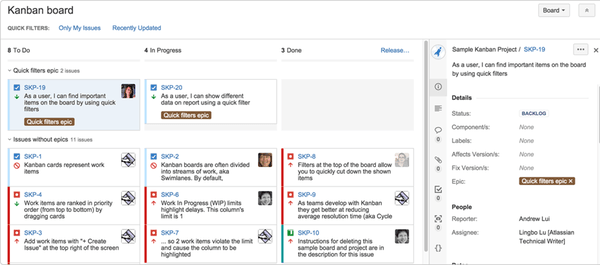
\includegraphics[width=1\textwidth]{fig/jira.png}
	\end{minipage}
	\caption{Interface JIRA}
	\label{fig:vdsadf}
\end{figure}
\subsubsection{GitLab}
GitLab est une application de gestion de dépôts git sous licence MIT. Elle permet d'héberger sur votre propre serveur des dépôts git avec l'interface web offrant tout le nécessaire pour vos projets : navigation dans le code source, suivi des demandes de bugs et d'évolutions (« issues »), wiki, gestion des droits d'accès par équipe, commentaires, notifications, etc.\\
Chaque dépôt créé via Gitlab est ensuite accessible avec n’importe quel client git présent sur votre machine, en HTTP, HTTPS ou SSH et pour chaque projet, tous les détails pour la connexion git sont clairement mis en avant, avec les lignes de commande nécessaires si besoin.\\
La gestion des groupes et des utilisateurs est très bien pensée et permet de correctement segmenter les projets que vous hébergez et le suivi d’activité permet de se tenir au courant des dernières modifications sur le code. \\
Outre ces fonctionnalités, Gitlab permet également de gérér l'intégration continue de projet.\\
GitLab est un outil très complet, facile à prendre en main et que n’importe qui peut installer sans avoir besoin de grandes connaissances.
\begin{figure}[H]
	\centering
	\begin{minipage}{12cm}
		\centering
		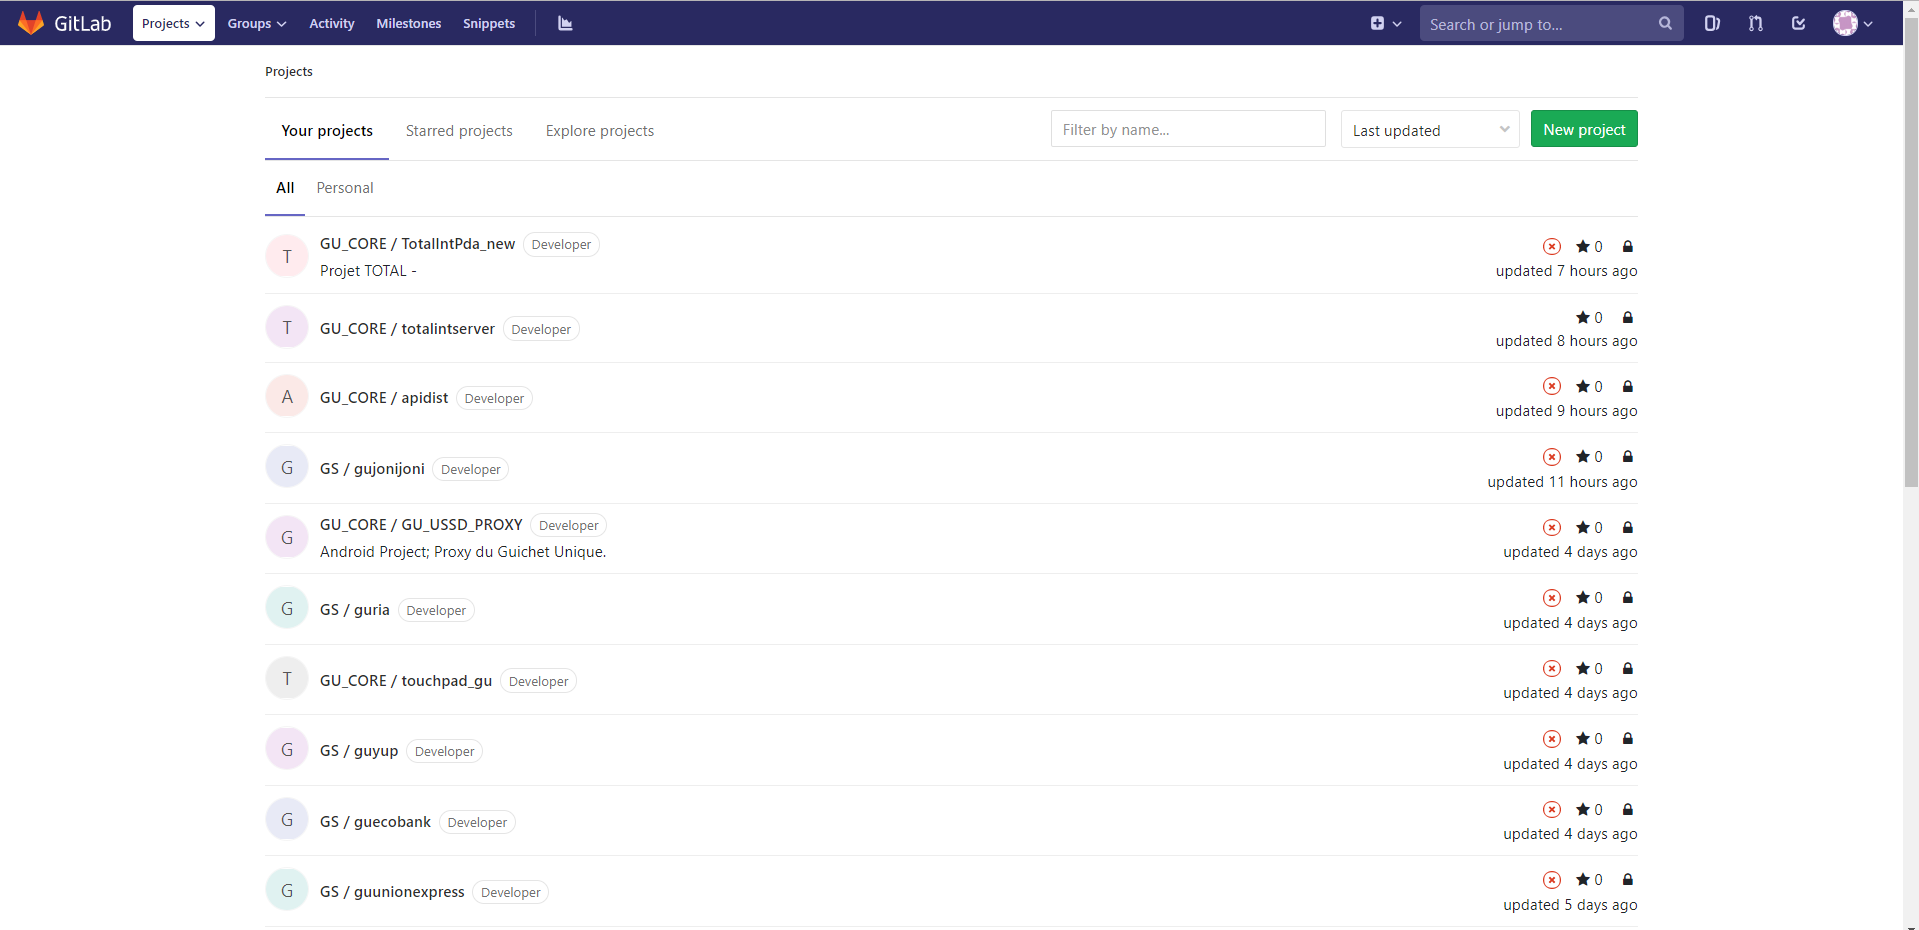
\includegraphics[width=1\textwidth]{fig/gitlab.png}
	\end{minipage}
	\caption{Repository GitLab de HubSo}
	\label{fig:vdsadf}
\end{figure}
\subsubsection{Jenkins}
L'intégration continue est un ensemble de pratiques utilisées en génie logiciel consistant à vérifier à chaque modification de code source que le résultat des modifications ne produit pas de régression dans l'application développée.\\
Jenkins, qui s'appelait à l'origine Hudson, est un outil d'Intégration Continue open source écrit en Java. Bénéficiant d'une part de marché dominante, Jenkins est utilisé par des équipes de toutes tailles, pour des projets dans des langages et des technologies variés, incluant .NET, Ruby, Groovy, Grails, PHP et d'autres, ainsi que Java bien sûr.\\
Jenkins présente de nombreux avantages :
\begin{itemize}
	\itemcheck Logiciel gratuit
	\itemcheck Plus de 1000 plugins sont disponibles
	\itemcheck Vous pouvez créer un plugin si celui que vous désirez n'existe pas
	\itemcheck Vous pouvez également partager ce plugin
	\itemcheck Logiciel facile à installer
\end{itemize}
\begin{figure}[H]
	\centering
	\begin{minipage}{12cm}
		\centering
		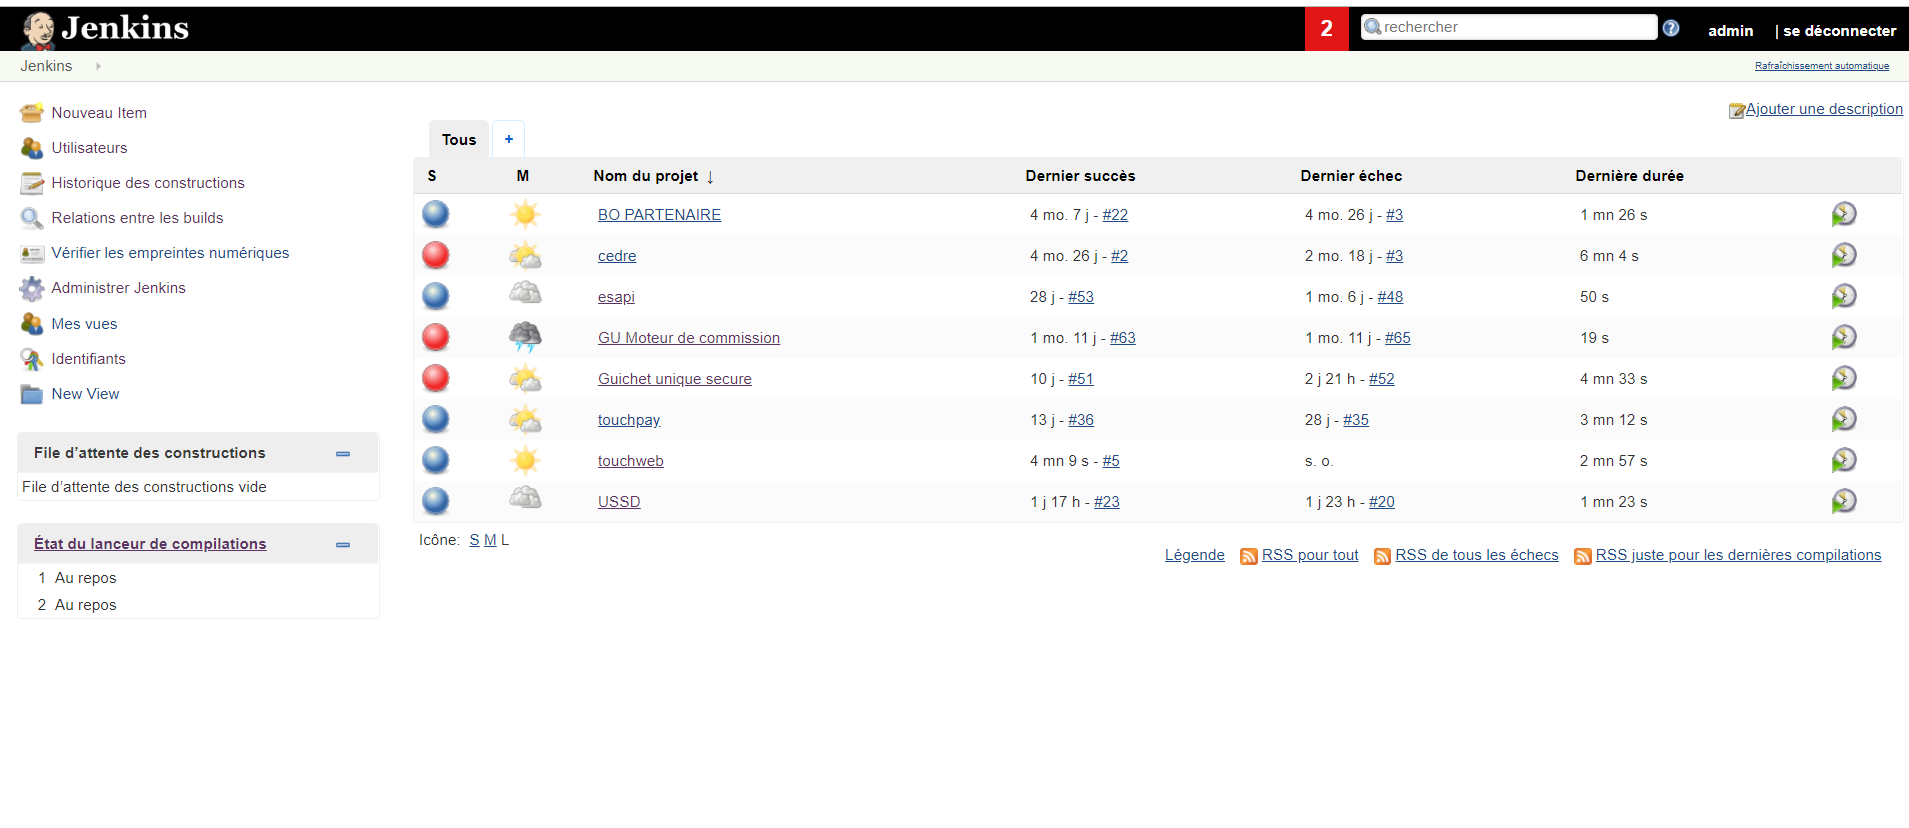
\includegraphics[width=1\textwidth]{fig/jenkins.png}
	\end{minipage}
	\caption{Instace Jenkins de HubSo}
	\label{fig:vadf}
\end{figure}
\subsubsection{Nexus}
Nexus est une plateforme de gestion de dépôts, permettant d'héberger des artéfacts. Ces artéfacts sont des composants, générés par exemple au build d'un projet, et déposés ensuite sur Nexus grâce à l'outil Maven. Cet outil a une forte dépendance envers Maven. L'intérêt de Nexus est de pouvoir partager des artéfacts avec les autres développeurs d'un projet, voir avec toute une communauté.\\
L'outil Nexus trouve sa place dans le processus d'intégration continue, en récupérant les artéfacts générés lors du build d'un projet sous Jenkins.  \\
Afin de pouvoir utiliser Nexus pour y déposer des artéfacts, il faut créer des dépôts. Un dépôt Nexus peut se définir comme un dossier où sont stockés des collections de binaires et d'artéfacts logiciels. Ces éléments pouvant être récupérés lors du build d'un projet. Il existe plusieurs type de dépôts :
\begin{itemize}
	\itemcheck Hosted : les dépôts créés par les utilisateurs ;
	\itemcheck proxy : dépôts dont le serveur Nexus est seulement un relais ;
	\itemcheck virtual : transformation d'un dépôt Maven1 en Maven2 ;
	\itemcheck group : un regroupement de dépôts sous une même URL.
\end{itemize}
Il existe deux types de dépôts pour les artéfacts créés par les utilisateurs :
\begin{itemize}
	\itemcheck un dépôt pour les releases : \\
	une release dans le contexte de Maven est une version fixe d'un projet. Elle représente le but qui était fixé au début du développement, c'est une version livrable du logicielle. Si de nouveaux développements viennent se rajouter à cette version, alors le projet change de version, et une nouvelle release sera générée à la fin des développements
	\itemcheck un dépôt pour les snapshots : \\
	Une version snapshot est une version en cours de développement, toutes les fonctionnalités n'étant pas terminées. Il pourra y avoir plusieurs snapshots pour une même version d'un projet.
\end{itemize}
\begin{figure}[H]
	\centering
	\begin{minipage}{12cm}
		\centering
		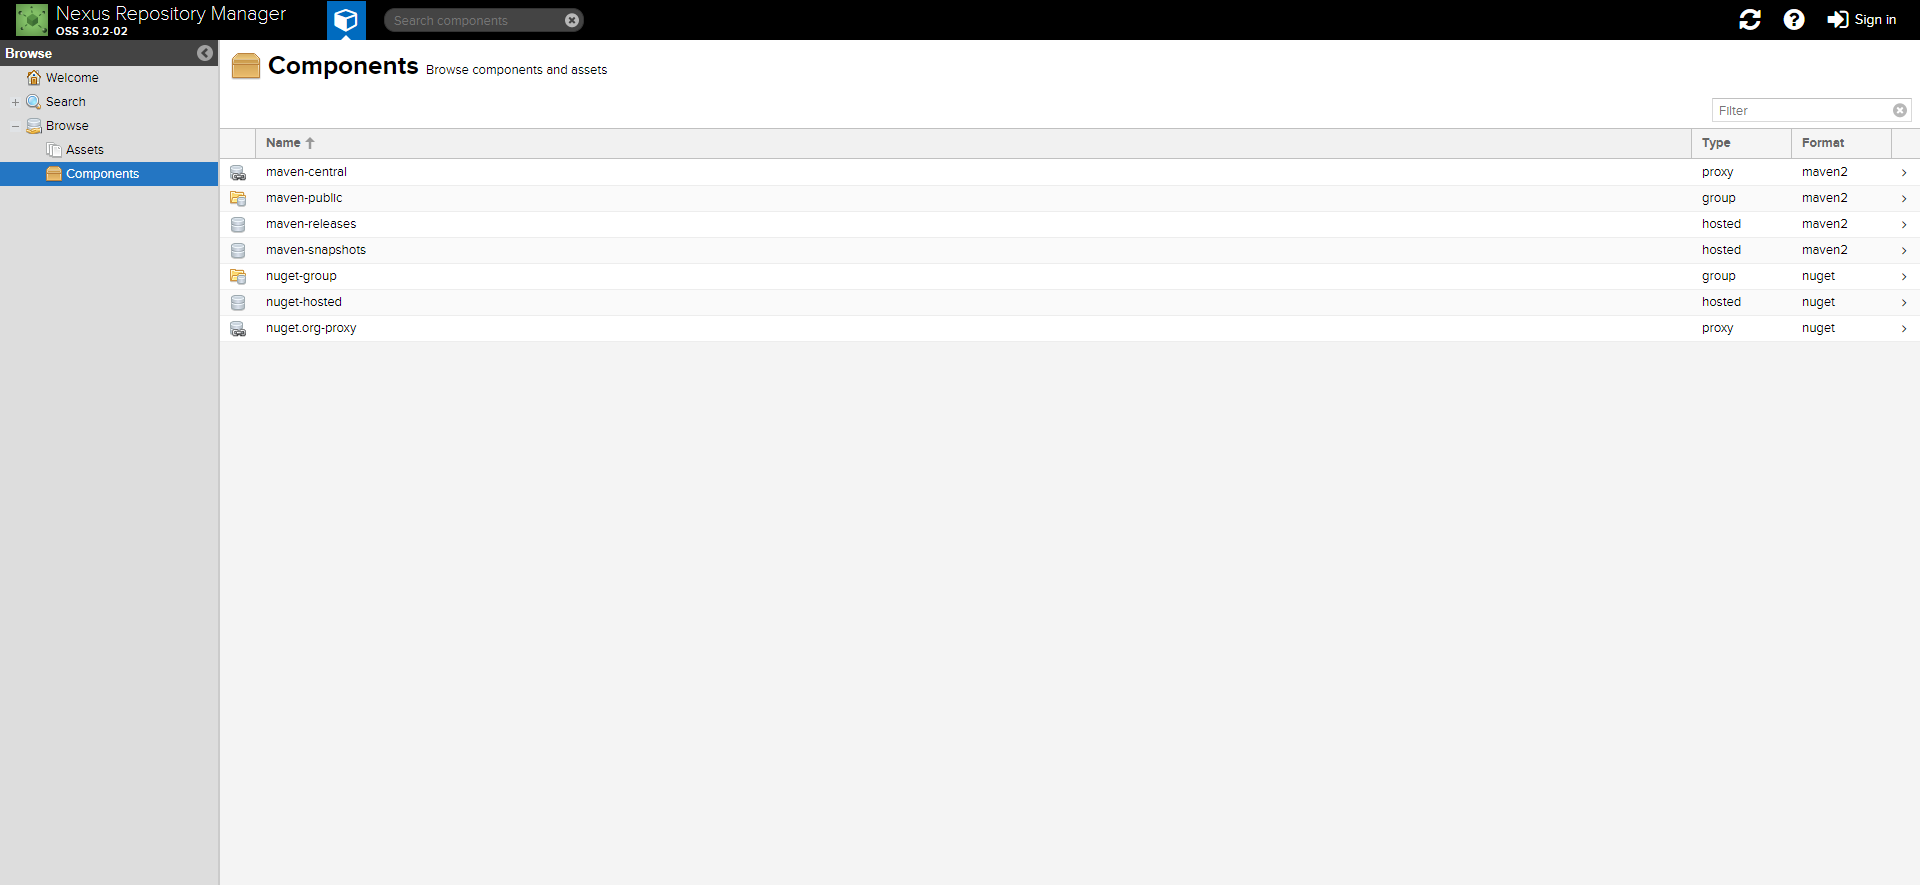
\includegraphics[width=1\textwidth]{fig/nexus.png}
	\end{minipage}
	\caption{Nexus Repository de HubSo}
	\label{fig:vdfdf}
\end{figure}
\subsubsection{SonarQube}
SonarQube (anciennement Sonar) est une plate-forme open source de contrôle continu de la qualité du code développée par SonarSource permettant d'effectuer des révisions automatiques avec analyse statique du code afin de détecter les bugs, les mauvaises pratiques et les failles de sécurité sur plus de 20 langages de programmation. SonarQube propose des rapports sur le code dupliqué, les normes de codage, les tests unitaires, la couverture de code, la complexité du code, les commentaires, les bugs et les vulnérabilités de sécurité.\\
SonarQube peut enregistrer l'historique des métriques et fournit des graphiques d'évolution. SonarQube fournit une analyse et une intégration entièrement automatisées avec  Maven, Ant, Gradle, MSBuild et des outils d'intégration continue tels que Jenkins.
SonarQube offre de nombreux avantages :
\begin{itemize}
	\itemcheck Tableau de bord complet des différents projets suivis
	\itemcheck Détection rapide du code à risque
	\itemcheck Support de plus de vingt-cinq langages (Java, C, C++, Objective-C, C\#, PHP, Flex, Groovy, JavaScript, Python, PL/SQL, COBOL…), dont certains sont sous licence commerciale
	\itemcheck Mesures quantitatives : nombre de classes, duplication de code, etc
	\itemcheck Support de plus de 600 règles de qualité
	\itemcheck Mesures qualitatives : couverture et taux de réussite des tests, complexité du code, respect des règles de codage, ...
	\itemcheck Gestion de profils pour les règles de codage.
	\itemcheck Visualisation du code source, surlignant les violations des règles de codage qui s'y trouvent.
	\itemcheck Historiques des statistiques, pour en voir l'évolution au cours du temps
	\itemcheck Analyses entièrement automatisées : intégration avec Maven, Ant, Gradle et serveurs d'intégration continue (Atlassian Bamboo, Jenkins, Hudson…).
	\itemcheck Intégration avec l'environnement de développement Eclipse
	\itemcheck Intégration avec des outils externes : Jira, Mantis, LDAP, Fortify…
	\itemcheck Support des plugins
	\itemcheck Implémentation de SQALE pour évaluer la dette technique.
	\itemcheck Reporting sur :
	\begin{itemize}
		\itemtirait identification des duplications de code
		\itemtirait mesure du niveau de documentation
		\itemtirait respect des règles de programmation
		\itemtirait détection des bugs potentiels
		\itemtirait évaluation de la couverture de code par les tests unitaires
		\itemtirait analyse de la répartition de la complexité
		\itemtirait analyse du design et de l'architecture d'une application
	\end{itemize}
\end{itemize}
\begin{figure}[H]
	\centering
	\begin{minipage}{12cm}
		\centering
		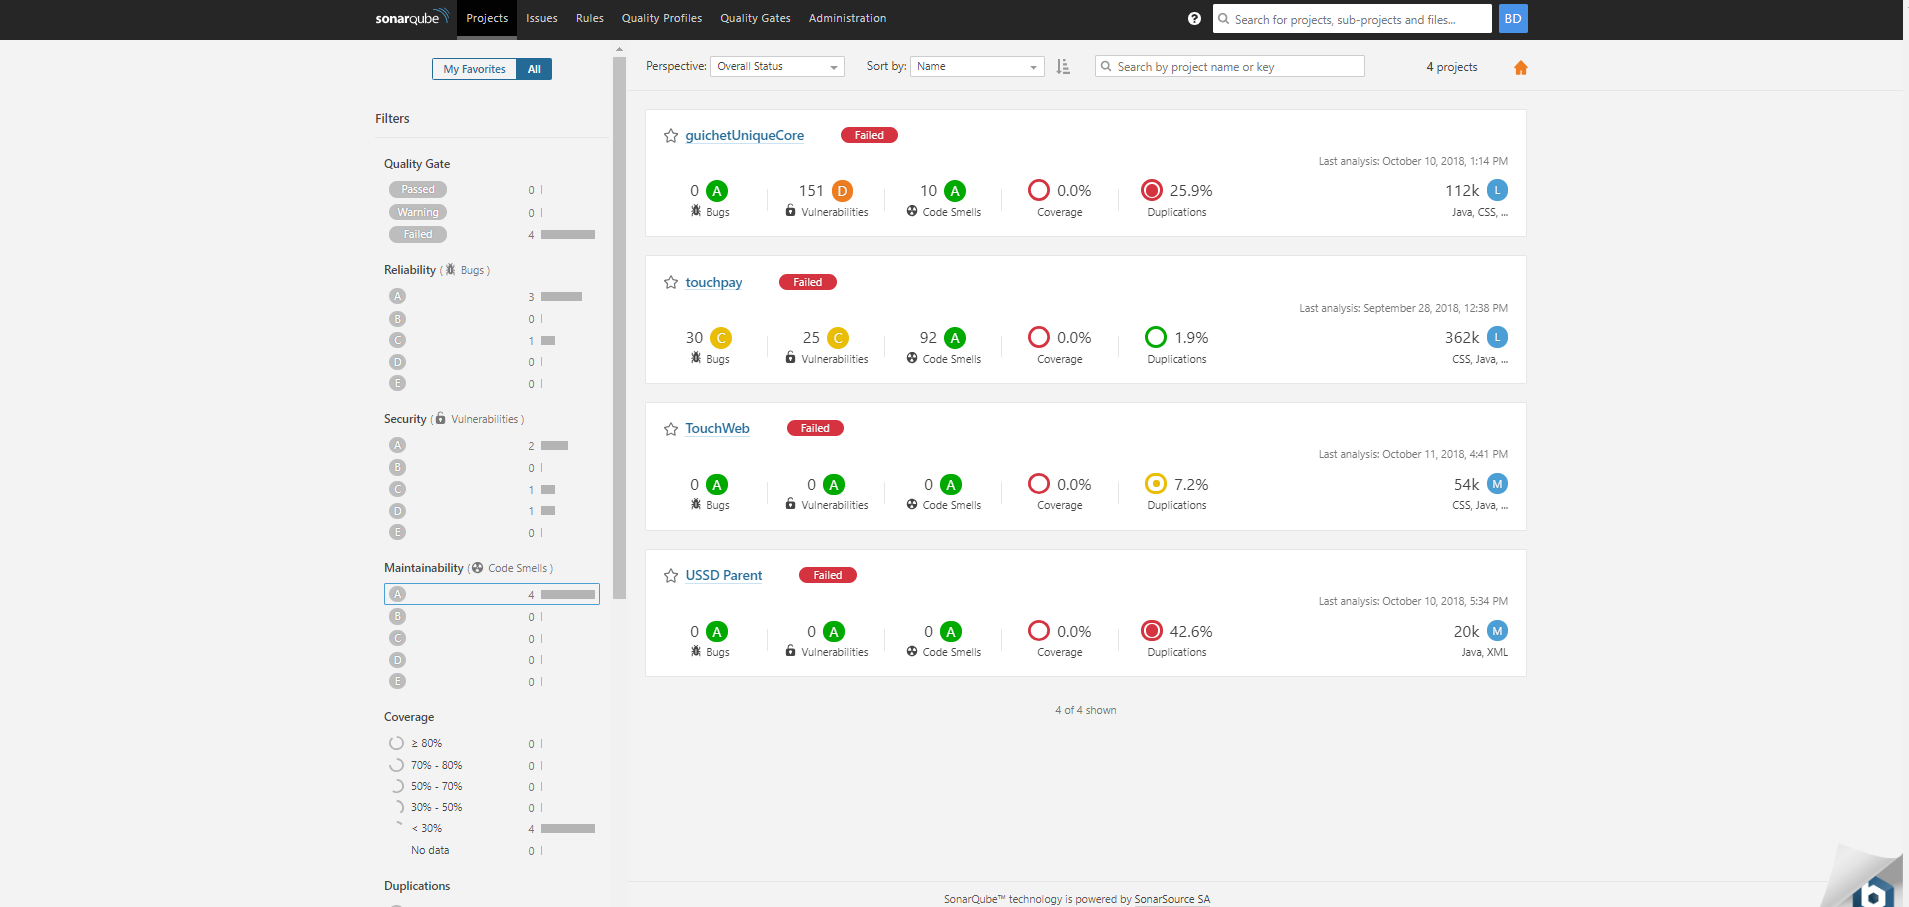
\includegraphics[width=1\textwidth]{fig/sonar.png}
	\end{minipage}
	\caption{Interface SonarQube de HubSo}
	\label{fig:vfdf}
\end{figure}
%TODO\section{Architecture fonctionnelle des applications utilisatrices de HubSo ESAPI}

\section{Mise en place de la bibliothèque HubSo ESAPI}
\subsection{Clonage de la bibliothèque OWASP ESAPI}
Nous avons débuté la mise en place de HubSo ESAPI en clônant le repository github du projet OWASP ESAPI. Il est accessible à l'adresse \textit{https://github.com/ESAPI/esapi-java-legacy}.
\begin{figure}[H]
	\centering
	\begin{minipage}{12cm}
		\centering
		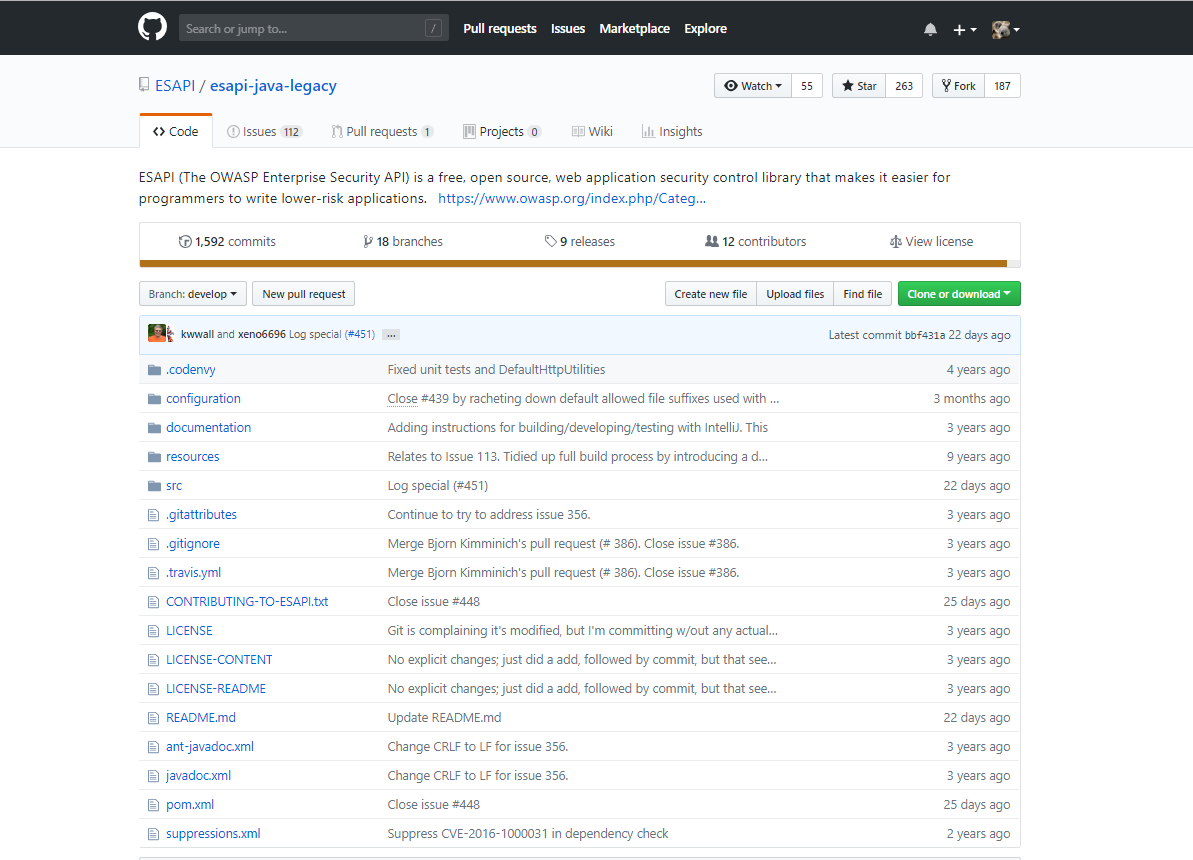
\includegraphics[width=1\textwidth]{fig/ESAPI-GIT.PNG}
	\end{minipage}
	\caption{Repository Github du projet OWASP ESAPI}
	\label{fig:vdf}
\end{figure}
Voici à quoi ressemble la bibliothèque ESAPI :
\begin{figure}[H]
	\centering
	\begin{minipage}{12cm}
		\centering
		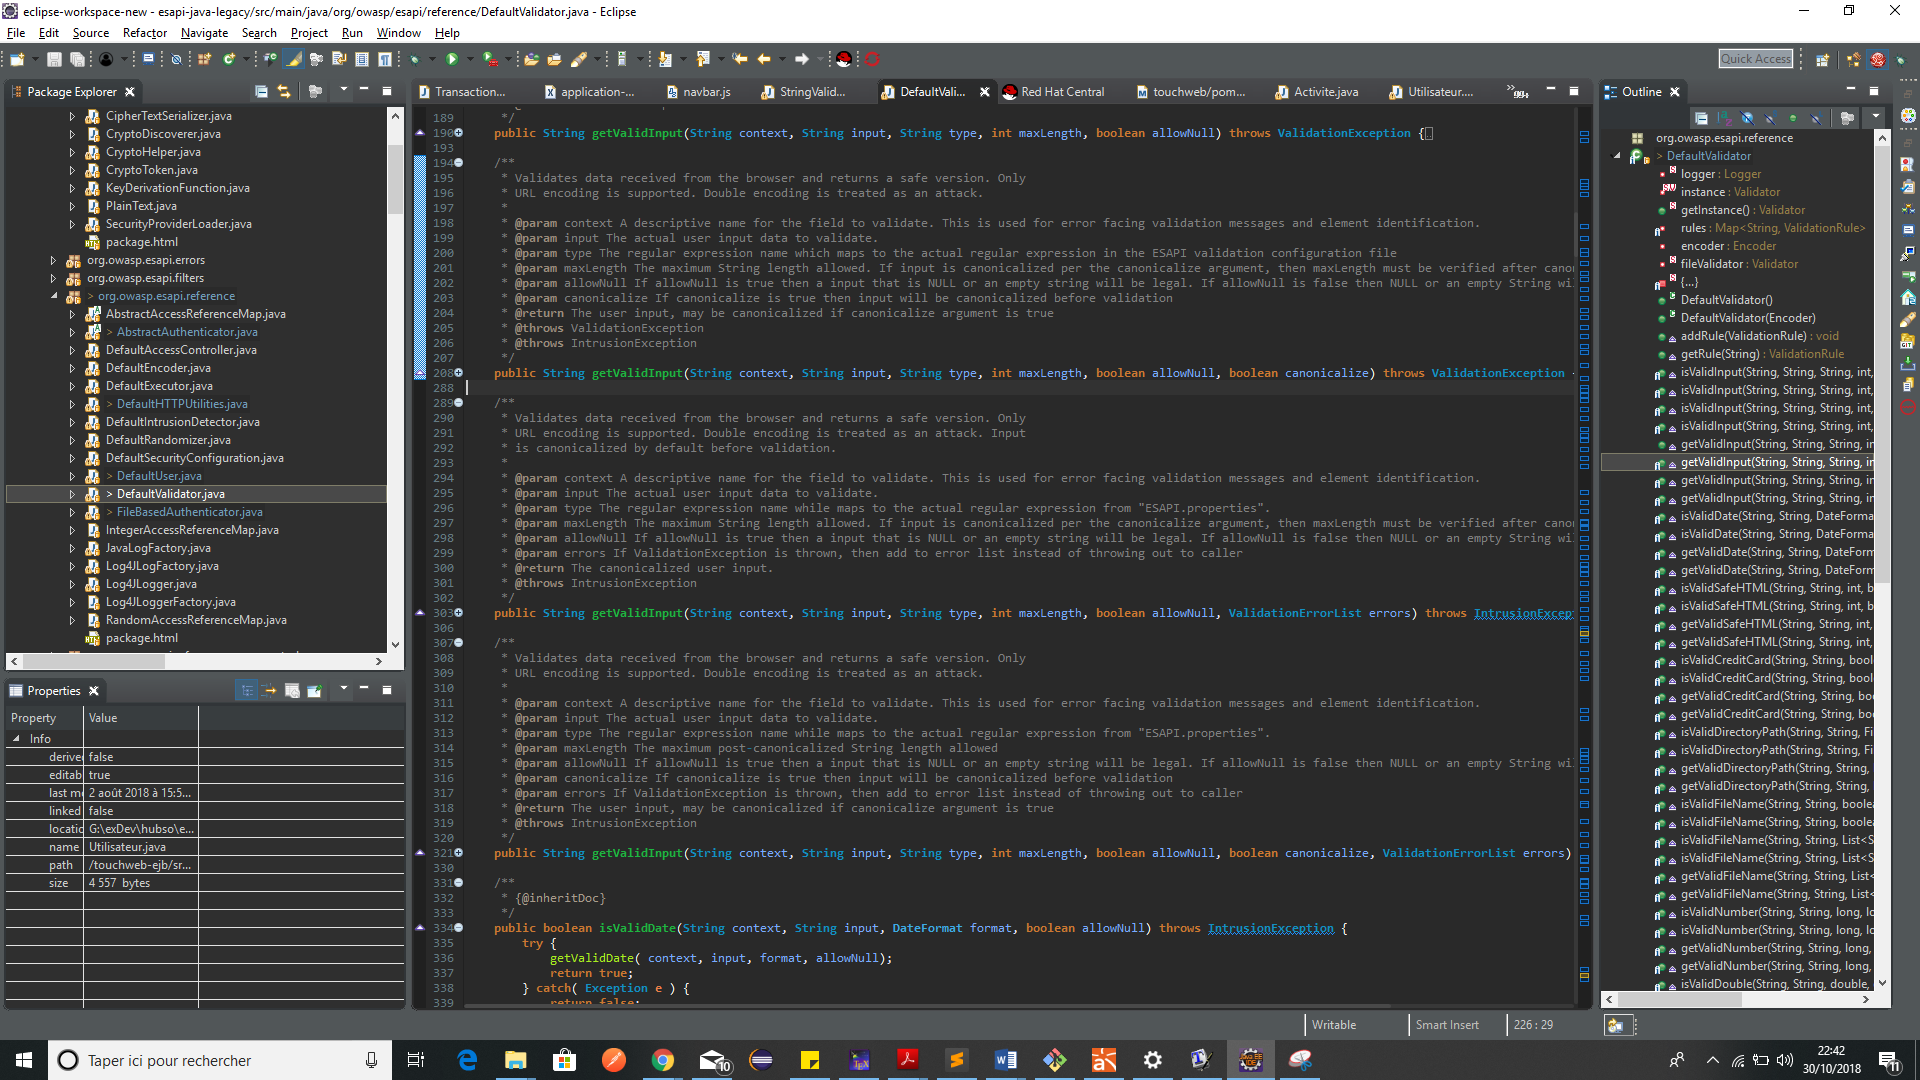
\includegraphics[width=1\textwidth]{fig/eclipse-esapi.png}
	\end{minipage}
	\caption{Bibliothèque HubSo ESAPI}
	\label{fig:vcdf}
\end{figure}
\subsection{Configuration}
L'implémentation de référence de la bibliothèque ESAPI utilise un répertoire «ressources» contenant plusieurs fichiers. Le répertoire des ressources peut être situé n’importe où sur le classpath ou peut être spécifié avec une variable d’environnement par ligne de commande comme suit: 
\begin{verbatim}
-D org.owasp.esapi.resources=”C:\resources” 
\end{verbatim}
Le fichier le plus important du répertoire est le fichier \textit{ESAPI.properties}. Dans ce fichier, on doit spécifier les différentes classes qui implémentent les différentes interfaces. Voici, ci-dessous, un extrait de ce fichier :
\lstset{language=Python}
\begin{lstlisting}
ESAPI.AccessControl=org.owasp.esapi.reference.DefaultAccessController
ESAPI.Authenticator=org.owasp.esapi.reference.FileBasedAuthenticator2
ESAPI.Encoder=org.owasp.esapi.reference.DefaultEncoder
ESAPI.Encryptor=org.owasp.esapi.reference.JavaEncryptor
ESAPI.CipherText=org.owasp.esapi.reference.DefaultCipherText
ESAPI.PreferredJCEProvider=SunJCE
ESAPI.Executor=org.owasp.esapi.reference.DefaultExecutor
ESAPI.HTTPUtilities=org.owasp.esapi.reference.DefaultHTTPUtilities
ESAPI.IntrusionDetector=org.owasp.esapi.reference.DefaultIntrusionDetector
ESAPI.Logger=org.owasp.esapi.reference.Log4JLogFactory2
ESAPI.Randomizer=org.owasp.esapi.reference.DefaultRandomizer
ESAPI.Validator=org.owasp.esapi.reference.DefaultValidator
\end{lstlisting}
On doit aussi configurer les différentes classes, ajouter des modèles de validation, les configurations de journalisation, les algorithmes de chiffrement et les seuils d'exception. Voici, ci-dessous un extrait de ce fichier par rapport à différentes configurations :
\begin{lstlisting}
# ESAPI Authenticator
Authenticator.AllowedLoginAttempts=3
Authenticator.MaxOldPasswordHashes=13
Authenticator.UsernameParameterName=username
Authenticator.PasswordParameterName=password
# RememberTokenDuration (in days)
Authenticator.RememberTokenDuration=14
# Session Timeouts (in minutes)
Authenticator.IdleTimeoutDuration=20
Authenticator.AbsoluteTimeoutDuration=120
# ESAPI Encoder
Encoder.DefaultCodecList=HTMLEntityCodec,PercentCodec,JavaScriptCode
# ESAPI Encryption
Encryptor.MasterKey=7AXyrRttFnPJHgzD/lTntA==
Encryptor.MasterSalt=tBp5pH+wXKHoICzUMLvnLQcncKE=
# AES is the most widely used and strongest encryption algorithm. This
# should agree with your Encryptor.CipherTransformation property.
Encryptor.EncryptionAlgorithm=AES
Encryptor.CipherTransformation=AES/CBC/PKCS5Padding
Encryptor.EncryptionKeyLength=128
# Valid values:		random|fixed|specified		'specified' not yet implemented; planned for 2.1n
Encryptor.ChooseIVMethod=random
Encryptor.fixedIV=0x000102030405060708090a0b0c0d0e0f
Encryptor.CipherText.useMAC=true
# Whether or not the PlainText object may be overwritten and then marked
# eligible for garbage collection. If not set, this is still treated as 'true'.
Encryptor.PlainText.overwrite=true
# Do not use DES except in a legacy situation. 56-bit is way too small key size.
#Encryptor.EncryptionKeyLength=56
#Encryptor.EncryptionAlgorithm=DES
Encryptor.HashAlgorithm=SHA-512
Encryptor.HashIterations=1024
Encryptor.DigitalSignatureAlgorithm=DSA
Encryptor.DigitalSignatureKeyLength=1024
Encryptor.RandomAlgorithm=SHA1PRNG
Encryptor.CharacterEncoding=UTF-8
# ESAPI HttpUtilties
HttpUtilities.UploadDir=C:\\ESAPI\\uploads
HttpUtilities.UploadTempDir=C:\\temp
# Force flags on cookies, if you use HttpUtilities to set cookies
HttpUtilities.ForceHttpOnlySession=false
HttpUtilities.ForceSecureSession=false
HttpUtilities.ForceHttpOnlyCookies=true
HttpUtilities.ForceSecureCookies=true
# File upload configuration
HttpUtilities.ApprovedUploadExtensions=.zip,.pdf,.doc,.docx,.ppt,.pptx,.tar,.gz,.tgz,.rar,.war,.jar,.ear,.xls,.rtf,.properties,.java,.class,.txt,.xml,.jsp,.jsf,.exe,.dll
HttpUtilities.MaxUploadFileBytes=500000000
HttpUtilities.ResponseContentType=text/html; charset=UTF-8
# ESAPI Executor
Executor.WorkingDirectory=C:\\Windows\\Temp
Executor.ApprovedExecutables=C:\\Windows\\System32\\cmd.exe,C:\\Windows\\System32\\runas.exe
# ESAPI Logging
# Set the application name if these logs are combined with other applications
Logger.ApplicationName=TouchWeb
Logger.LogEncodingRequired=true
Logger.LogApplicationName=true
Logger.LogServerIP=false
Logger.LogFileName=ESAPI_logging_file
Logger.MaxLogFileSize=50000
# ESAPI Intrusion Detection
IntrusionDetector.event.test.count=2
IntrusionDetector.event.test.interval=10
IntrusionDetector.event.test.actions=disable,log
IntrusionDetector.org.owasp.esapi.errors.IntrusionException.count=1
IntrusionDetector.org.owasp.esapi.errors.IntrusionException.interval=1
IntrusionDetector.org.owasp.esapi.errors.IntrusionException.actions=log,disable,logout
IntrusionDetector.org.owasp.esapi.errors.IntegrityException.count=10
IntrusionDetector.org.owasp.esapi.errors.IntegrityException.interval=5
IntrusionDetector.org.owasp.esapi.errors.IntegrityException.actions=log,disable,logout
org.owasp.esapi.errors.ValidationException.count=10
org.owasp.esapi.errors.ValidationException.interval=10
org.owasp.esapi.errors.ValidationException.actions=log,logout
IntrusionDetector.org.owasp.esapi.errors.AuthenticationHostException.count=2
IntrusionDetector.org.owasp.esapi.errors.AuthenticationHostException.interval=10
IntrusionDetector.org.owasp.esapi.errors.AuthenticationHostException.actions=log,logout
# ESAPI Validation
# The ESAPI Validator works on regular expressions with defined names. You can define names
# either here, or you may define application specific patterns in a separate file defined below.
# This allows enterprises to specify both organizational standards as well as application specific
# validation rules.
Validator.ConfigurationFile=validation.properties
# Validators used by ESAPI
Validator.AccountName=^[a-zA-Z0-9]{3,20}$
Validator.SystemCommand=^[a-zA-Z\\-\\/]{1,64}$
Validator.RoleName=^[a-z]{1,20}$
# Global HTTP Validation Rules
# Values with Base64 encoded data (e.g. encrypted state) will need at least [a-zA-Z0-9\/+=]
Validator.HTTPScheme=^(http|https)$
Validator.HTTPServerName=^[a-zA-Z0-9_.\\-]*$
Validator.HTTPParameterName=^[a-zA-Z0-9_]{1,32}$
Validator.HTTPParameterValue=^[a-zA-Z0-9.\\-\\/+=_ ]*$
Validator.HTTPCookieName=^[a-zA-Z0-9\\-_]{1,32}$
Validator.HTTPCookieValue=^[a-zA-Z0-9\\-\\/+=_ ]*$
Validator.HTTPHeaderName=^[a-zA-Z0-9\\-_]{1,32}$
Validator.HTTPHeaderValue=^[a-zA-Z0-9()\\-=\\*\\.\\?;,+\\/:&_ ]*$
Validator.HTTPContextPath=^[a-zA-Z0-9.\\-_]*$
Validator.HTTPPath=^[a-zA-Z0-9.\\-_]*$
Validator.HTTPQueryString=^[a-zA-Z0-9()\\-=\\*\\.\\?;,+\\/:&_ ](1,50)$
Validator.HTTPURI=^[a-zA-Z0-9()\\-=\\*\\.\\?;,+\\/:&_ ]*$
Validator.HTTPURL=^.*$
Validator.HTTPJSESSIONID=^[A-Z0-9]{10,30}$
# Validation of file related input
Validator.FileName=^[a-zA-Z0-9!@#$%^&{}\\[\\]()_+\\-=,.~'` ]{1,255}$
Validator.DirectoryName=^[a-zA-Z0-9:/\\\\!@#$%^&{}\\[\\]()_+\\-=,.~'` ]{1,255}$
\end{lstlisting}
Un autre fichier important est le fichier \textit{Validation.properties}. C'est dans ce fichier qu'on définit les modèles de validation. Une fois définie ici, la validation d'une donnée d'un type présent ici se fait par rapport au regex correspondant. Ci dessous, un extrait de ce fichier :
\begin{lstlisting}
Validator.SafeString=[A-Za-z0-9]{0,1024}$
Validator.Email=^[A-Za-z0-9._%-]+@[A-Za-z0-9.-]+\\.[a-zA-Z]{2,4}$
Validator.CreditCard=^(\\d{4}[- ]?){3}\\d{4}$
Validator.SSN=^(?!000)([0-6]\\d{2}|7([0-6]\\d|7[012]))([ -]?)(?!00)\\d\\d\\3(?!0000)\\d{4}$
Validator.SenegaleseMobilePhoneNumber=^7[0|6|7|8][0-9]{7}$
Validator.IPAddress=^(?:(?:25[0-5]|2[0-4][0-9]|[01]?[0-9][0-9]?)\\.){3}(?:25[0-5]|2[0-4][0-9]|[01]?[0-9][0-9]?)$
Validator.URL=^(ht|f)tp(s?)\\:\\/\\/[0-9a-zA-Z]([-.\\w]*[0-9a-zA-Z])*(:(0-9)*)*(\\/?)([a-zA-Z0-9\\-\\.\\?\\,\\:\\'\\/\\\\\\+=&amp;%\\$#_]*)?$
\end{lstlisting}
\subsection{Déploiement}
Après avoir configuré ESAPI, il faut le rendre disponible aux autres applications. Pour ce faire, nous l'avons déployé dans le Nexus repository de HubSo comme suit :
\lstset{language=XML}
\begin{lstlisting}
<distributionManagement>
	<repository>
		<id>nexus</id>
		<url>http://nexus.xerus.hubso.net/repository/maven-releases/</url>
	</repository>
	<snapshotRepository>
		<id>nexus</id>
		<url>http://nexus.xerus.hubso.net/repository/maven-snapshots/</url>
	</snapshotRepository>
</distributionManagement>
\end{lstlisting}
Voici l'artéfact esapi à présent disponible aux applications dans le Nexus Repository
\begin{figure}[H]
	\centering
	\begin{minipage}{12cm}
		\centering
		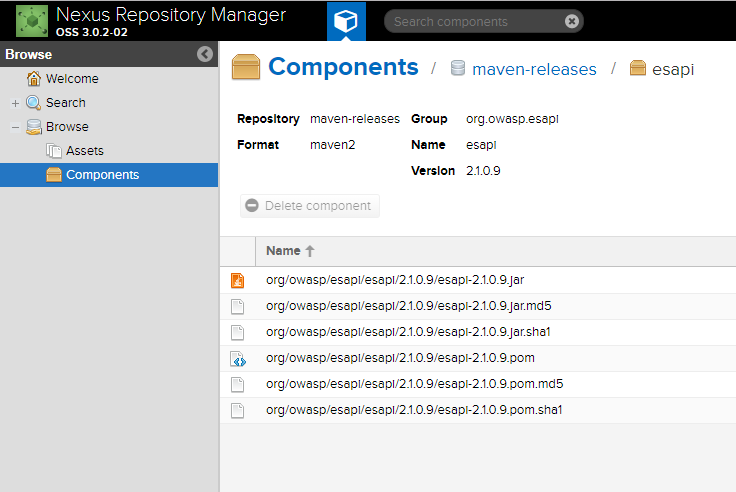
\includegraphics[width=1\textwidth]{fig/nexus-esapi.png}
	\end{minipage}
	\caption{Artéfact esapi dans le Nexus Repository de HubSo}
	\label{fig:vccdf}
\end{figure}
\section{Intégration de HubSo ESAPI dans TouchWeb}
Après avoir mise en place la bibliothèque, nous allons l'éprouver en l'utilisant dans une application existante ; TouchWeb. TouchWeb est une solution permettant de faire de multiples opérations :
\begin{itemize}
	\itemcheck Transfert de crédit Orange, Tigo, Expresso ;
	\itemcheck Mobile Money Orange Money, Tigo Cash, Vitfé, Wizall ;
	\itemcheck Transfert d'argent Joni Joni, Ria ;
	\itemcheck Paiement de factures Woyofal, Senelec
	\itemcheck Paiement d'autres services tels que les assurances ;
	\itemcheck Autres opérations.
\end{itemize}
L'on voit ainsi les enjeux de cette application et à quel point la sécurité y est primordiale.\\
Ainsi, nous avons intégré la bibliothèque de sécurité à TouchWeb. La bibliothèque étant déjà disponible sur le repository Nexus, cela se fait par un simple ajout de dépendance Maven dans le \textit{pom.xml} parent du projet TouchWeb.
\begin{figure}[H]
	\centering
	\begin{minipage}{12cm}
		\centering
		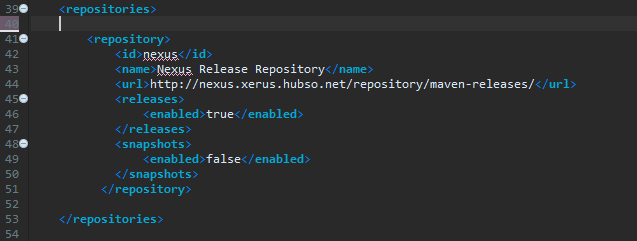
\includegraphics[width=1\textwidth]{fig/nexus-repository.png}
	\end{minipage}
	\caption{Ajout du repository Nexus contenant l'artéfact esapi}
	\label{fig:vccdfs}
\end{figure}
\begin{figure}[H]
	\centering
	\begin{minipage}{12cm}
		\centering
		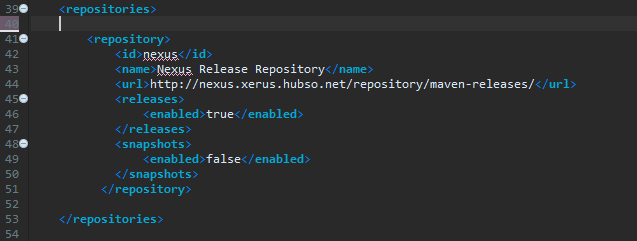
\includegraphics[width=1\textwidth]{fig/nexus-repository.png}
	\end{minipage}
	\caption{Ajout de la dépendance esapi parmi les dépendances du projet TouchWeb}
	\label{fig:vccdfs}
\end{figure}
On peut maintenant commencer à utiliser les fonctions de sécurité disponibles dans la bibliothèque.
\subsection{État initial}
Pour commencer, nous allons créer un projet Jenkins qui nous permettra d'automatiser certaines tâches pour nous telles que l'analyse Sonar. Pour ce faire, nous créons un job «touchweb». \\
Ce job est configuré de la sorte :
\begin{itemize}
	\itemcheck La scrutation de code source se fait sur le repository GitLab de HubSo correspondant ;
	\itemcheck Un build est déclenché lorsqu'il y a modification au niveau du repository GitLab. La scrutation du code source se fait toutes les quinze minutes ;
	\itemcheck L'environnement de build est «Maven Release Build» ;
	\itemcheck Le goal de build est le suivant :
	\begin{verbatim}
		clean install -P xerus,!kazan
	\end{verbatim}
	\itemcheck A la suite du build, l'analyse avec SonarQube est déclenchée.
\end{itemize} 
\begin{figure}[H]
	\centering
	\begin{minipage}{12cm}
		\centering
		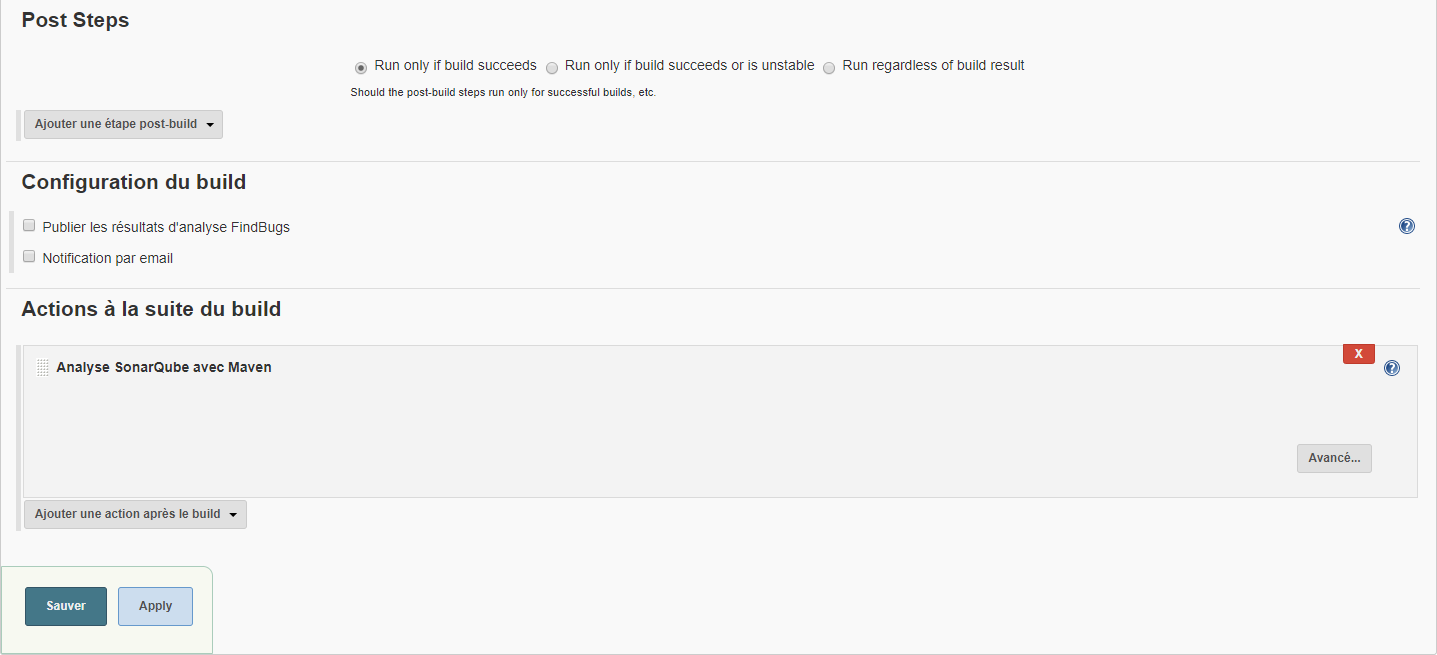
\includegraphics[width=1\textwidth]{fig/sonar-post-action.png}
	\end{minipage}
	\caption{Déclenchement analyse SonarQube après un build réussi}
	\label{fig:vccdfxdfs}
\end{figure}
La revue de code manuelle afin de trouver les bugs de sécurité n'étant pas très aisée, nous allons nous aider de Sonar. En effet, Sonar dispose d'un plug-in appelé «FindBugs» qui fonctionne très bien avec les projets développés en Java. FindBugs génère des rapports (Security Reports) par rapport au Top 10 OWASP mais aussi au Top 25 Sans. C'est un plugin très reconnu et utilisé par les équipes d'audit de sécurité. 
\begin{figure}[H]
	\centering
	\begin{minipage}{12cm}
		\centering
		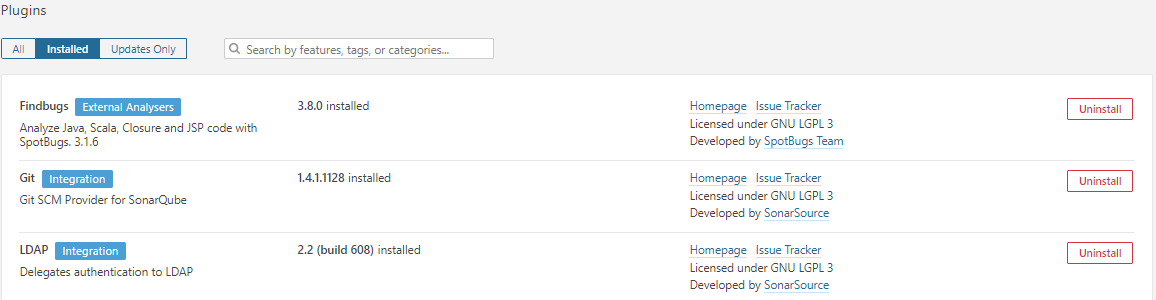
\includegraphics[width=1\textwidth]{fig/findbugs-plugin.png}
	\end{minipage}
	\caption{Configuration repository GitLab distant}
	\label{fig:vccdfxdfs}
\end{figure}
Le plug-in «FindBugs» nous permet d'avoir plusieurs profils de revue de code orientés sécurité. Nous allons utiliser le profil «FindBugs Security Audit» qui est le profil orienté sécurité le plus élevé. Il fait carrément un audit de sécurité.
\begin{figure}[H]
	\centering
	\begin{minipage}{12cm}
		\centering
		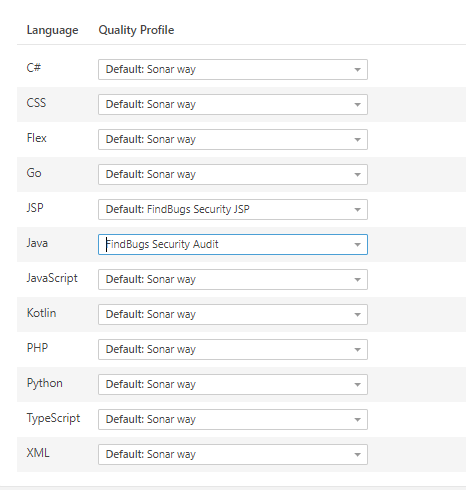
\includegraphics[width=1\textwidth]{fig/findbugs-profile.png}
	\end{minipage}
	\caption{Profil FindBugs Security Audit}
	\label{fig:sdfds}
\end{figure}
Après un premier audit sonar, voici que nous avons :
\begin{figure}[H]
	\centering
	\begin{minipage}{12cm}
		\centering
		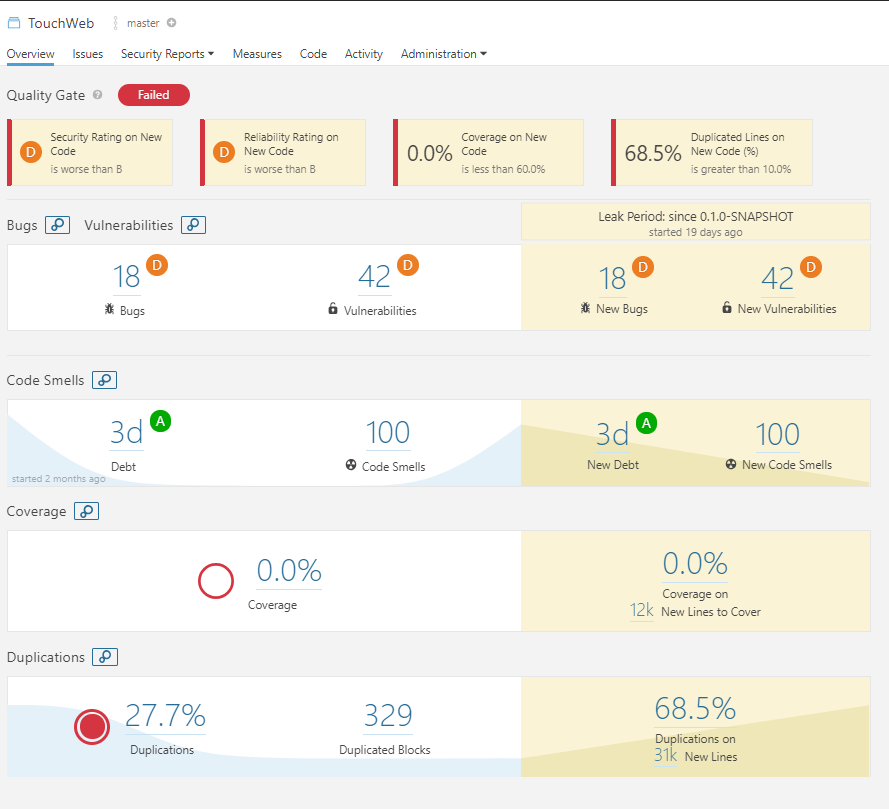
\includegraphics[width=1\textwidth]{fig/touchweb-first-sonar.PNG}
	\end{minipage}
	\caption{Premier audit Sonar de TouchWeb avec le profil FindBugs Security Audit}
	\label{fig:sddffds}
\end{figure}
L'analyse Sonar révèle qu'il y a 18 bugs et 42 vulnérabilités dans le projet. De ce fait, la note de sécurité est mauvaise ; on a un \textit{D} (la meilleure note est \textit{A}). Quand on essaie d'y voir de plus près, on se rend compte que parmi les 42 vulnérabilités, 3 sont critiques et 35 sont majeurs.
\begin{figure}[H]
	\centering
	\begin{minipage}{12cm}
		\centering
		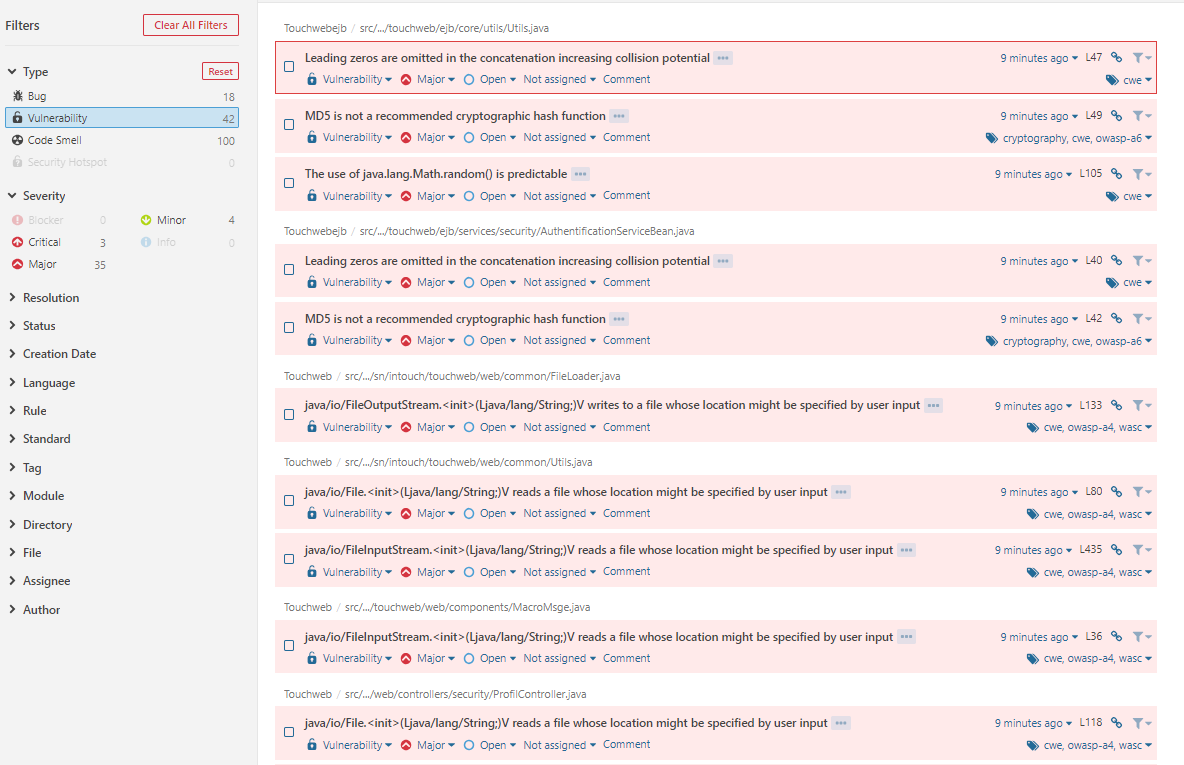
\includegraphics[width=1\textwidth]{fig/touchweb-first-overview.PNG}
	\end{minipage}
	\caption{Vulnérabilités TouchWeb}
	\label{fig:sdfdsds}
\end{figure}
Notre travail consiste maintenant à régler ces problèmes et obtenir une application plus sûre par l'utilisation de notre solution.
\subsection{Corrections}
La correction de TouchWeb s'est faite en prenant problème pour problème. Pour chaque vulnérabilité, Sonar préconise un contrôle à faire, il peut s'agir d'une validation à faire, d'un changement d'algorithme ou encore d'un encodage. Les actions faites nombreuses, nous allons juste en présenter quelques-unes.
\begin{figure}[H]
	\centering
	\begin{minipage}{12cm}
		\centering
		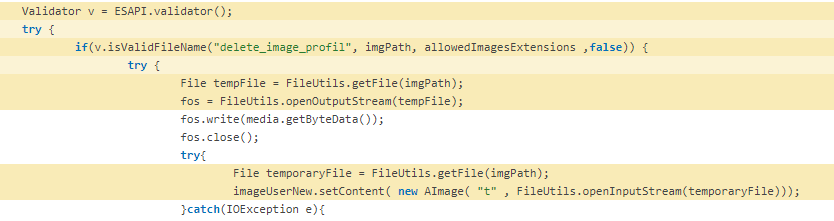
\includegraphics[width=1\textwidth]{fig/esapi-validation.PNG}
	\end{minipage}
	\caption{Validation avec HubSo ESAPI }
	\label{fig:sdfgdsds}
\end{figure}
L'envoi des requêtes HTTP se fait désormais en Digest comme suit :
\lstset{language=Java}
\begin{lstlisting}
public static JsonObject sendRequest(Parameter urlParam, String urlplus, String httpVerb, JsonObject jo) {

	logger.info("Json object sent : " + jo);

	String url = urlParam.getValue() + urlplus;

	logger.info("Absolute url " + url);

	JsonObject joRep = null;


	final DigestAuthenticator authenticator = new DigestAuthenticator( new Credentials("x","y"));
	final Map<String, CachingAuthenticator> authCache = new ConcurrentHashMap<String, CachingAuthenticator>();
	
	OkHttpClient.Builder builder = new OkHttpClient.Builder().readTimeout(2L* 60, TimeUnit.SECONDS)
	.connectTimeout(60, TimeUnit.SECONDS)
	.authenticator(new CachingAuthenticatorDecorator(authenticator, authCache))
	.addInterceptor(new AuthenticationCacheInterceptor(authCache));

	if (urlParam.getIsEncoded() == 0) {
		String proxyPort = null;
		String proxyHost = null;
		try {
			proxyPort = parameterService.getParameter("PROXY_PORT_WL").getValue().trim();
			proxyHost = parameterService.getParameter("PROXY_HOST_WL").getValue().trim();
		} catch (Exception e) {
			logger.info("###### Erreur recuperation proxy port et proxy host ##### :" +url + ":" + proxyPort + "/" + proxyHost );
		}
		if (proxyPort != null && proxyHost != null) {
			System.out.println("##### Using Proxy #####");
			Proxy proxy = new Proxy(Proxy.Type.HTTP, new InetSocketAddress(proxyHost, Integer.parseInt(proxyPort)));
			builder.proxy(proxy);
		}
	}

	final OkHttpClient client = builder.build();

	okhttp3.MediaType mediaType = okhttp3.MediaType.parse("application/json");

	RequestBody body = null;

	if(jo!=null) {
		body = RequestBody.create(mediaType, jo.toString());
	}

	Builder reqBuilder = new Request.Builder().url(url);
	if(httpVerb=="GET") {
		reqBuilder.get();
	}
	if(httpVerb=="POST") {
		reqBuilder.post(body);
	}
	if(httpVerb=="PUT") {
		reqBuilder.put(body);
	}
	if(httpVerb=="PATCH") {
		reqBuilder.patch(body);
	}
	if(httpVerb=="DELETE") {
		reqBuilder.delete(body);
	}

	Request request = reqBuilder.build();

	try {
		Response response = client.newCall(request).execute();
		if (response != null) {
			String codeResponse = response.networkResponse().code() + "";
			String responseBody = response.body().string();
			logger.info("TOUCH API RESPONSE CODE: " + codeResponse);
			logger.info("TOUCH API RESPONSE BODY: " + responseBody);
			if (response.code() == 200) {
				joRep = getJson(responseBody);
			}
		}
	} catch (IOException e) {
		logger.error("", e);
	}
	return joRep;
}
\end{lstlisting}
De même, lors de toute requête au serveur, l'adresse MAC de la machine hôte est envoyée et certaines opérations se font sur la base de la vérification de cette adresse MAC par rapport à celle uilisée lors de la connexion.
\begin{figure}[H]
	\centering
	\begin{minipage}{12cm}
		\centering
		
\includegraphics[width=1\textwidth]{fig/conn-mac.PNG}
	\end{minipage}
	\caption{Adresse MAC enregistrée à la connexion}
	\label{fig:sdedffds}
\end{figure}
Aussi, la connexion se fait à double facteur ; en plus du login et mot de passe,  un token est demandé. Ce token est préalablement généré et envoyé par sms sur le téléphone mobile de l'utilisateur.
\begin{figure}[H]
	\centering
	\begin{minipage}{12cm}
		\centering
		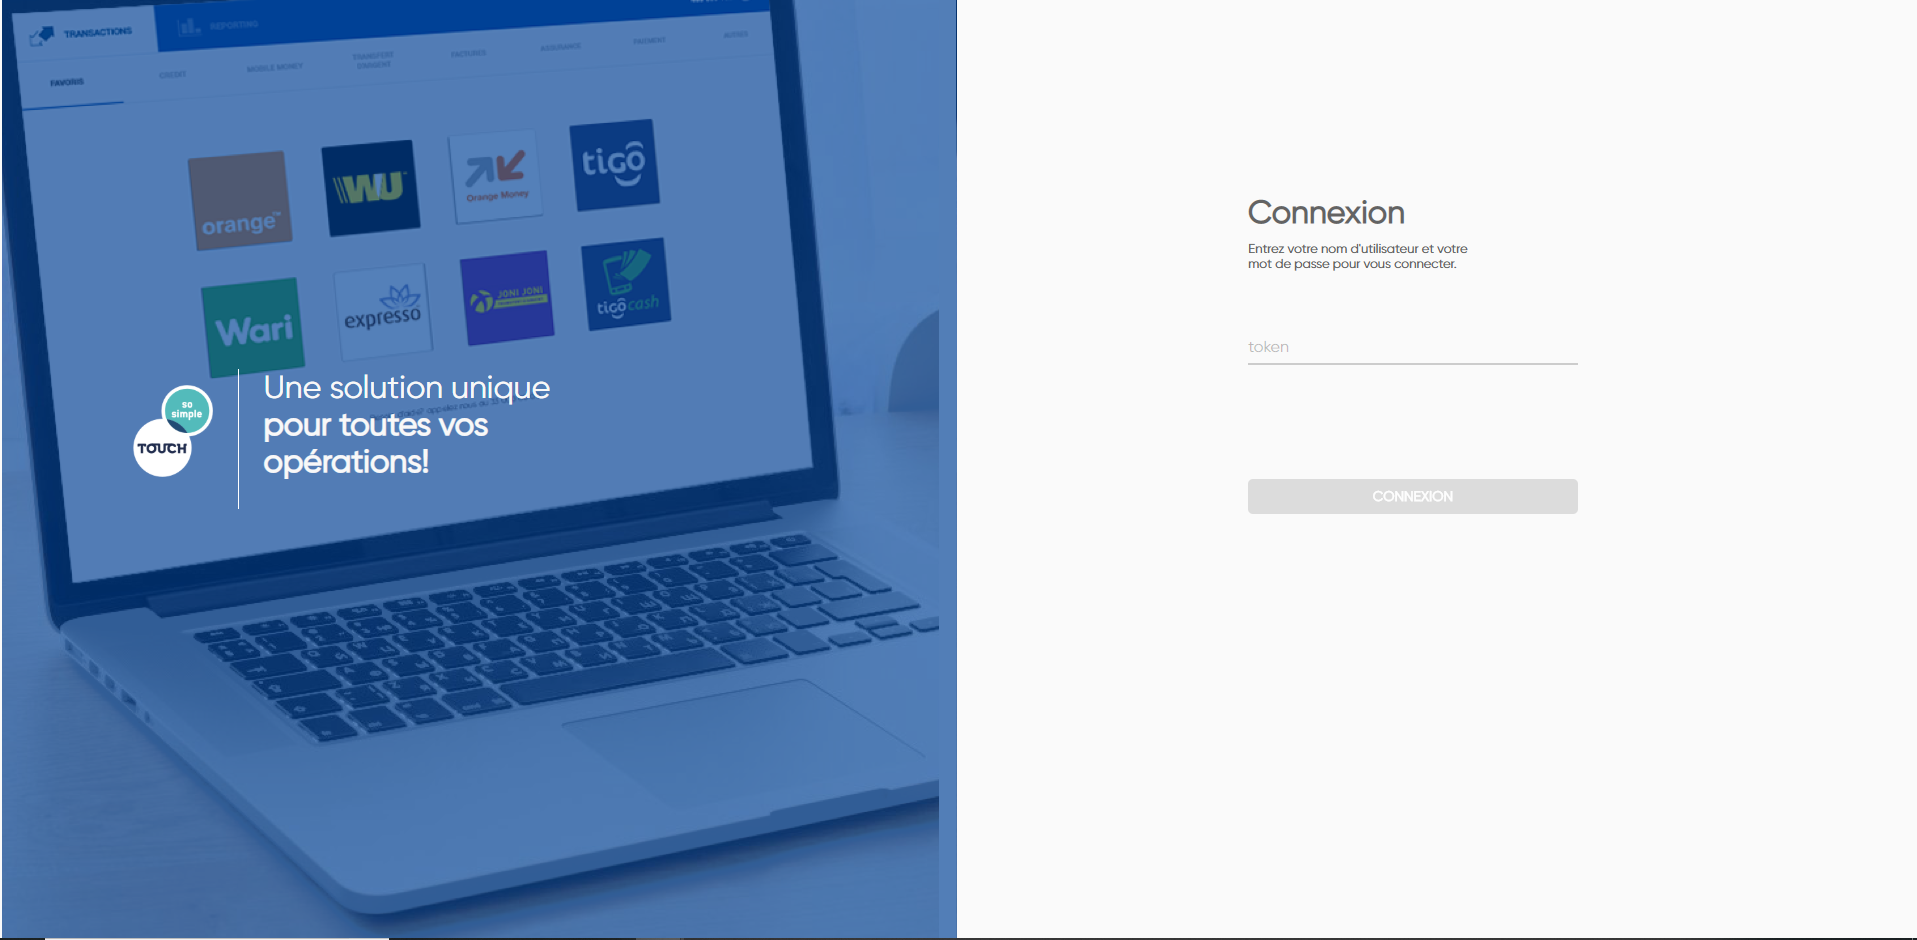
\includegraphics[width=1\textwidth]{fig/token.PNG}
	\end{minipage}
	\caption{Demande du token comme deuxième facteur}
	\label{fig:sdedffds}
\end{figure}
L'utilisateur ne peut accéder à l'application que si le token entré est bien celui qui a été généré.
\begin{figure}[H]
	\centering
	\begin{minipage}{12cm}
		\centering
		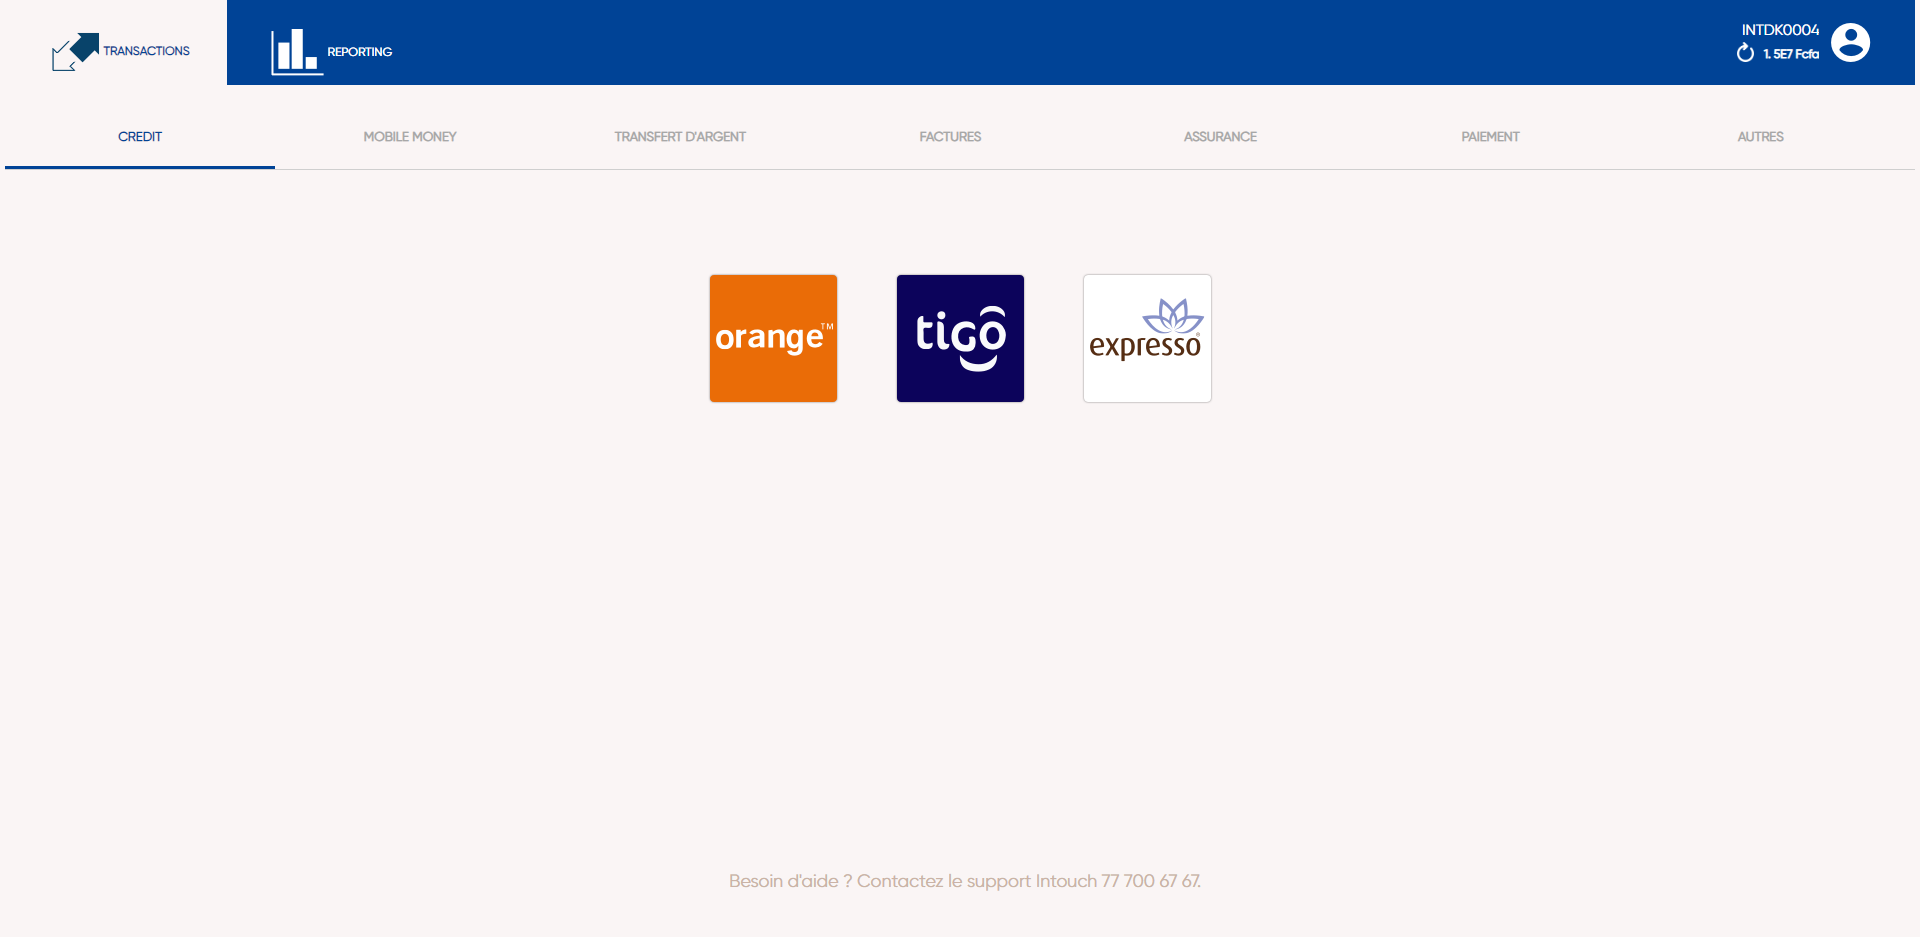
\includegraphics[width=1\textwidth]{fig/conn-ok.PNG}
	\end{minipage}
	\caption{Connexion réussie}
	\label{fig:sdedffds}
\end{figure}
Après un certain nombre de tentatives de connexion infructueuses, le compte de l'utilisateur est bloqué pour des raisons de sécurité.
\begin{figure}[H]
	\centering
	\begin{minipage}{12cm}
		\centering
		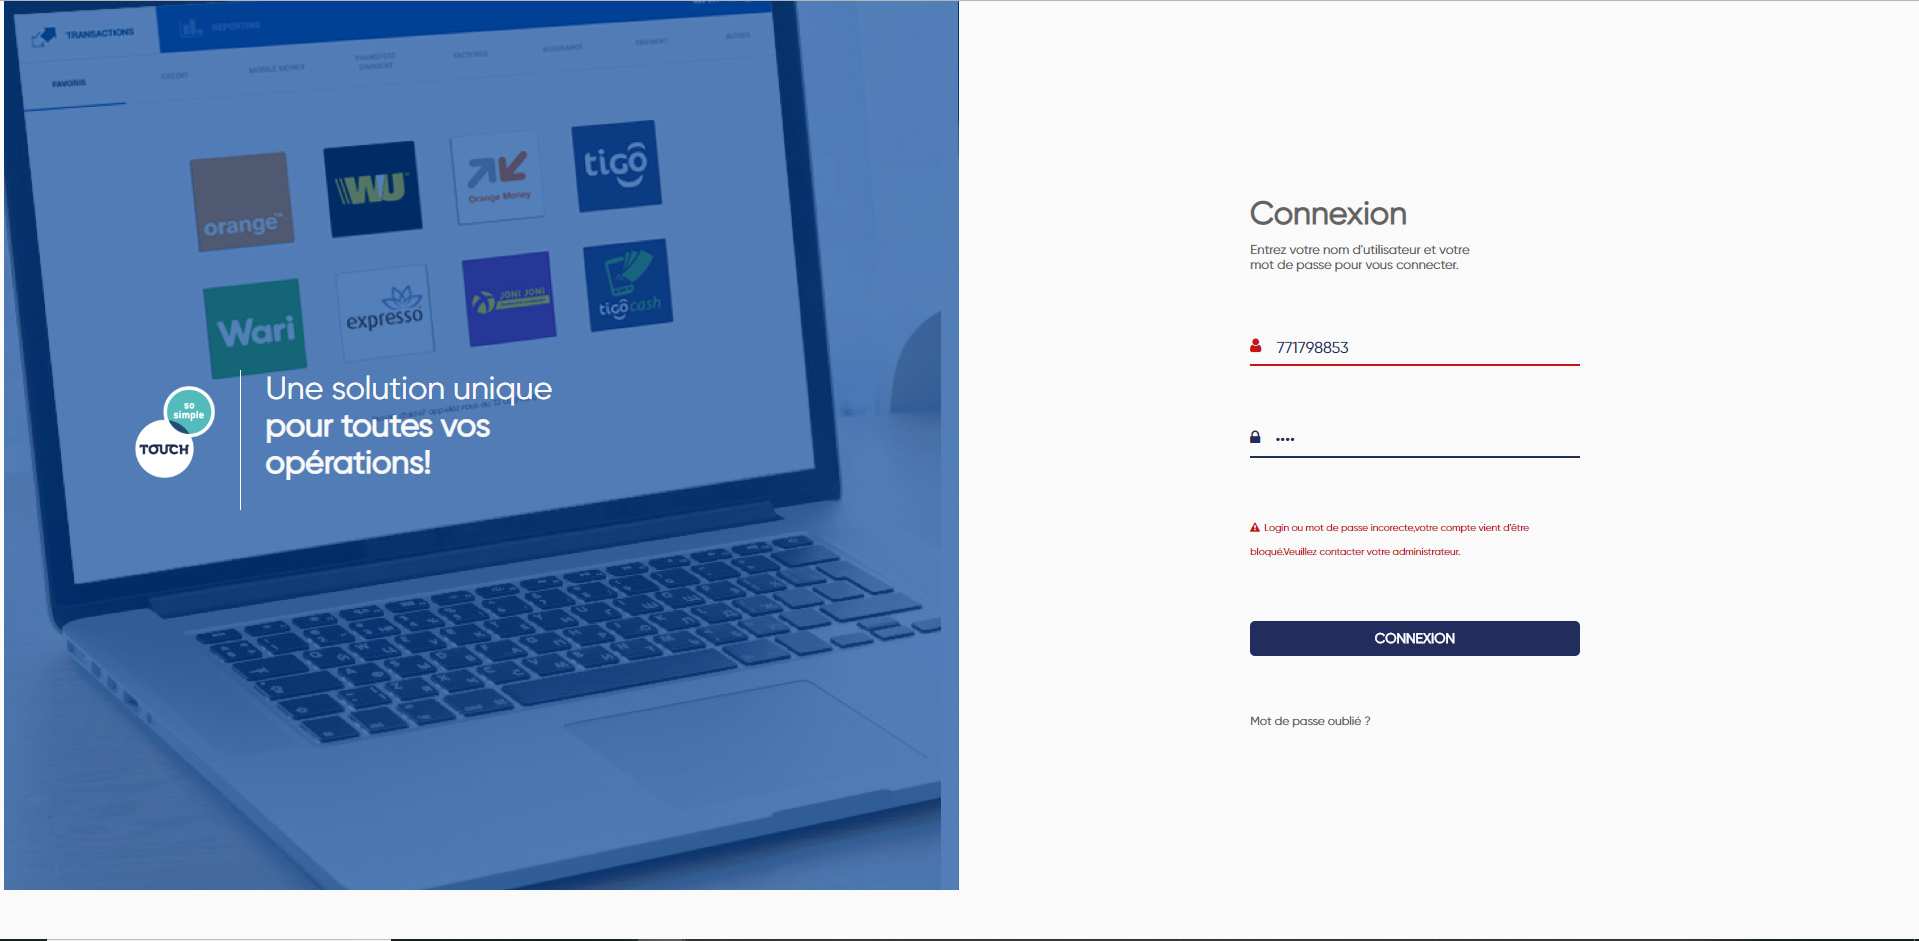
\includegraphics[width=1\textwidth]{fig/compte-bloque.PNG}
	\end{minipage}
	\caption{Compte bloqué}
	\label{fig:sfds}
\end{figure}
\subsection{État final}
Aprés avoir amené différents correctifs sur TouchWeb, nous avons constaté une nette amélioration.
En effet, nous avons maintenant une note \textit{A}, la meilleure note. De même, le nombre de vulnérabilités est de 0 ainsi que le nombre de bugs.
\begin{figure}[H]
	\centering
	\begin{minipage}{12cm}
		\centering
		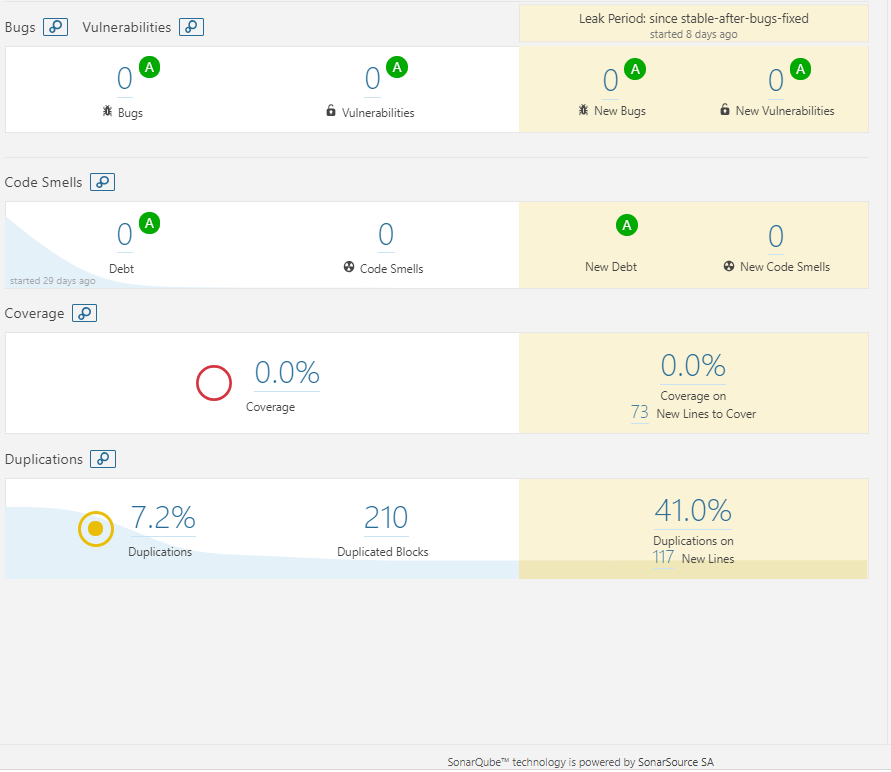
\includegraphics[width=1\textwidth]{fig/Capture1.PNG}
	\end{minipage}
	\caption{Correction TouchWeb}
	\label{fig:sfds}
\end{figure}
Le diagramme suivant montre l'évolution des vulnérabilités dans TouchWeb
\begin{figure}[H]
	\centering
	\begin{minipage}{12cm}
		\centering
		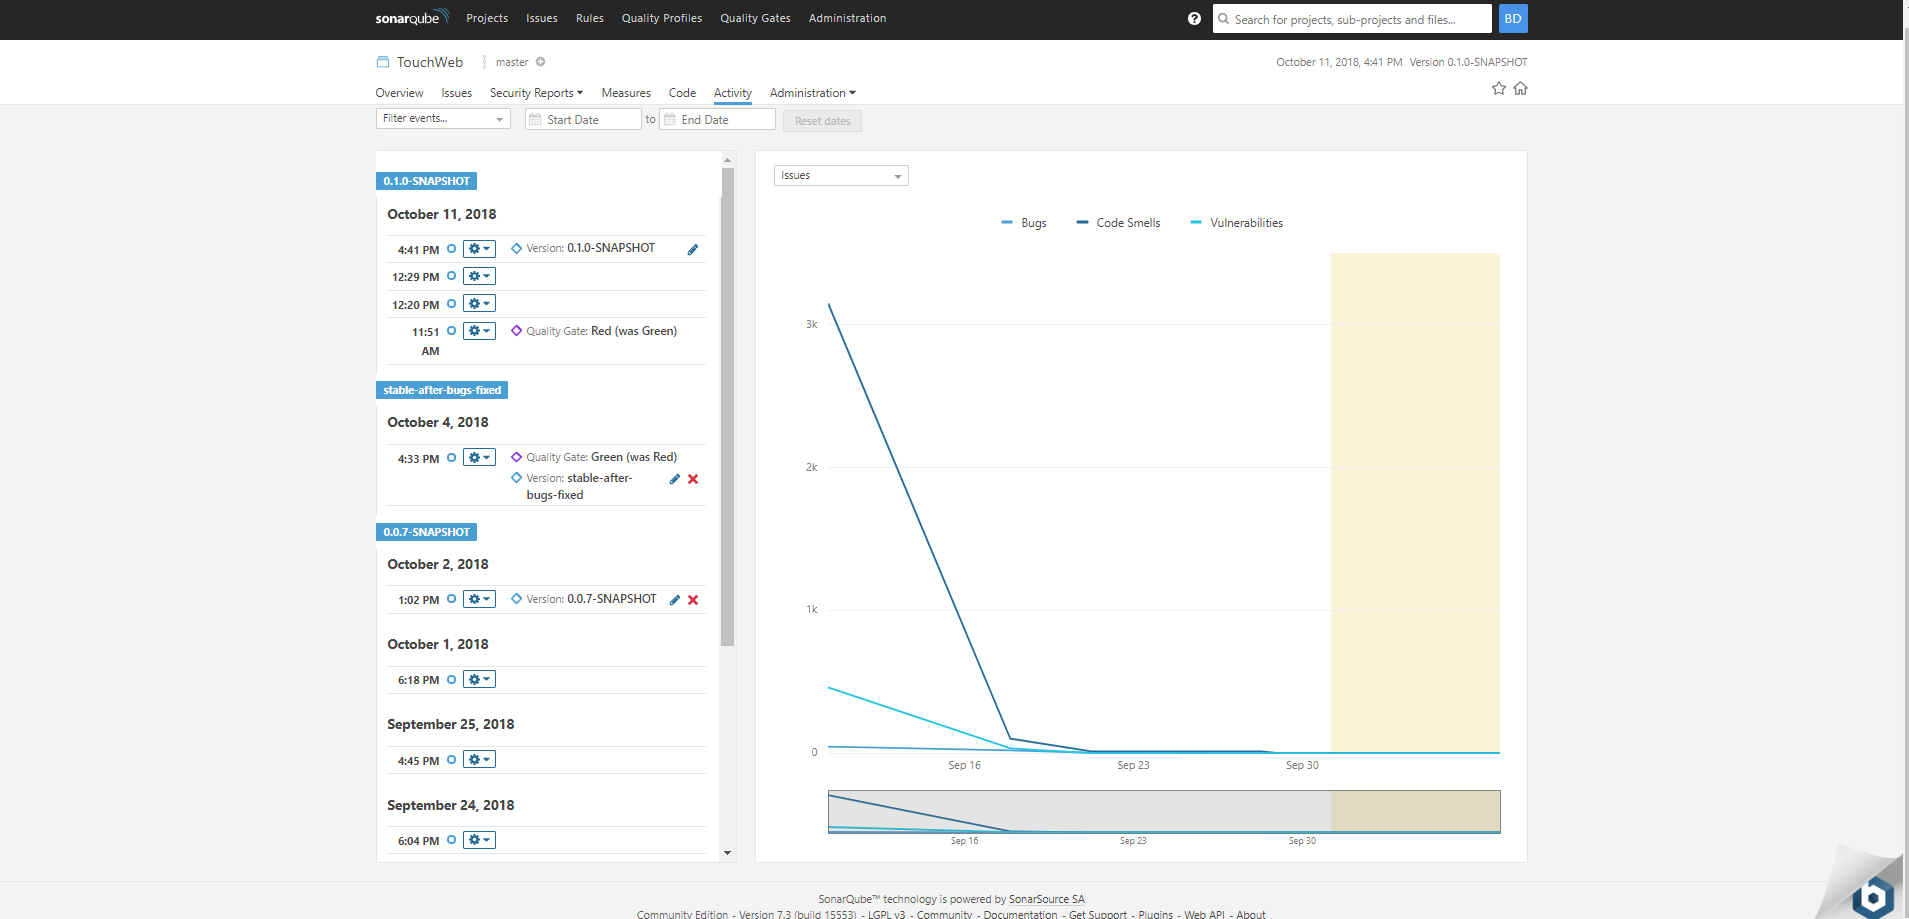
\includegraphics[width=1\textwidth]{fig/issues_diagram.png}
	\end{minipage}
	\caption{Evolution des vulnérabilités dans TouchWeb}
	\label{fig:sfds}
\end{figure}
On voit que les vulnérabilités et bugs ont baissé jusqu'à disparaître pour le moment.\\
La figure suivante montre les différentes notes allouées aux différents fichiers source et on voit que nous avons des \textit{A} partout.
\begin{figure}[H]
	\centering
	\begin{minipage}{12cm}
		\centering
		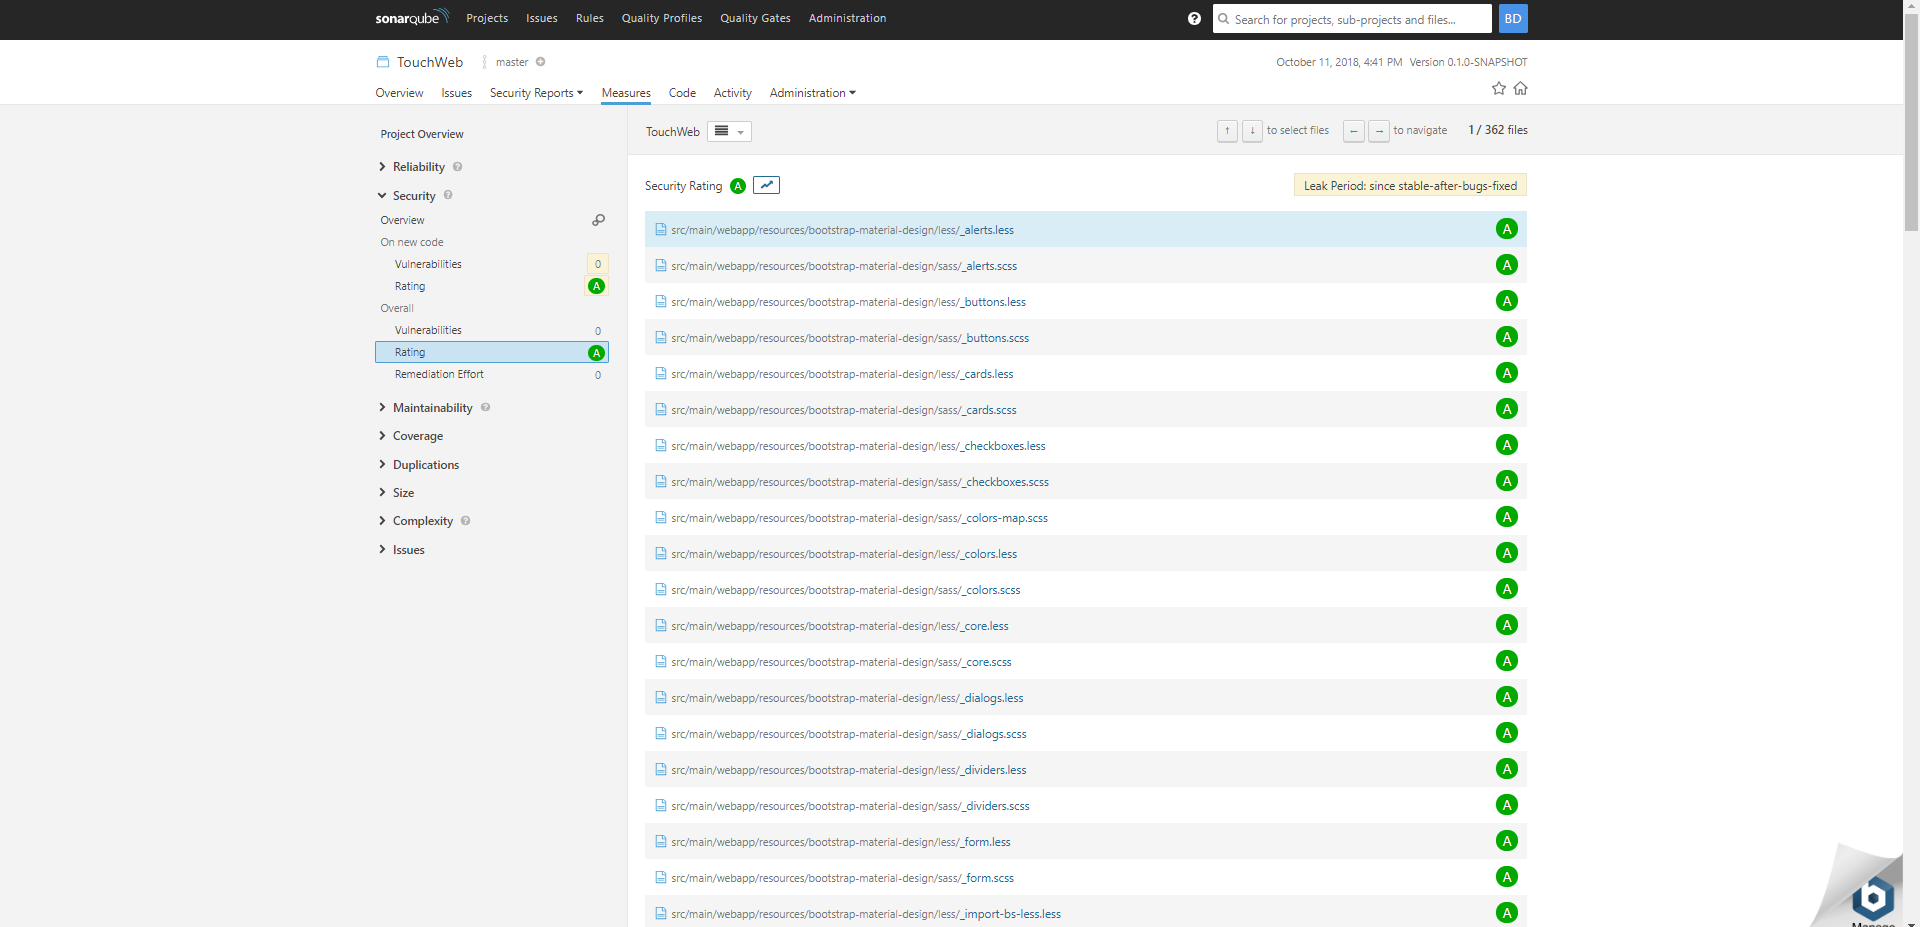
\includegraphics[width=1\textwidth]{fig/security_rating.png}
	\end{minipage}
	\caption{Notes des fichiers source}
	\label{fig:sfds}
\end{figure}
De même, les rapports Owasp Top 10 et Sans Top 25 sont rassurants et que le projet est conforme à ces rapports.
\begin{figure}[H]
	\centering
	\begin{minipage}{12cm}
		\centering
		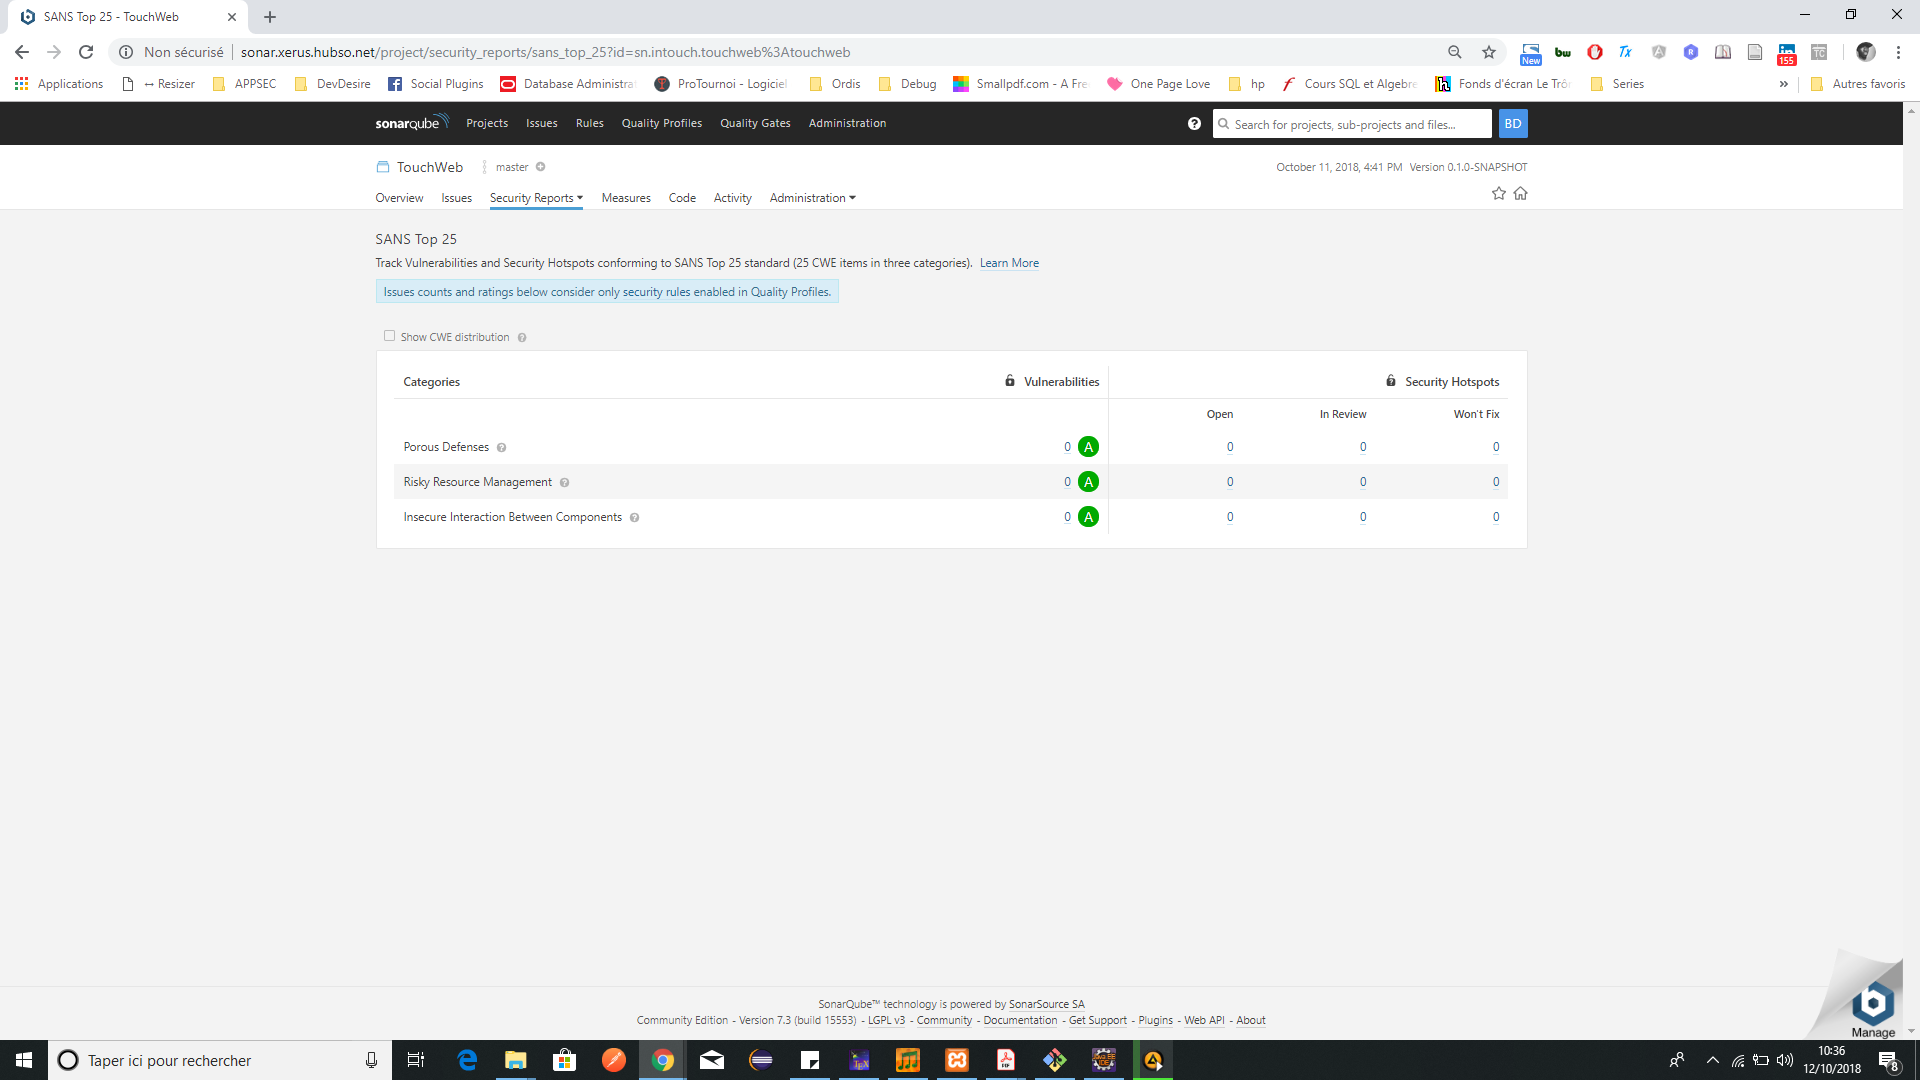
\includegraphics[width=1\textwidth]{fig/Sans_top_25.png}
	\end{minipage}
	\caption{Rapport Sans Top 25}
	\label{fig:sfds}
\end{figure}
\begin{figure}[H]
	\centering
	\begin{minipage}{12cm}
		\centering
		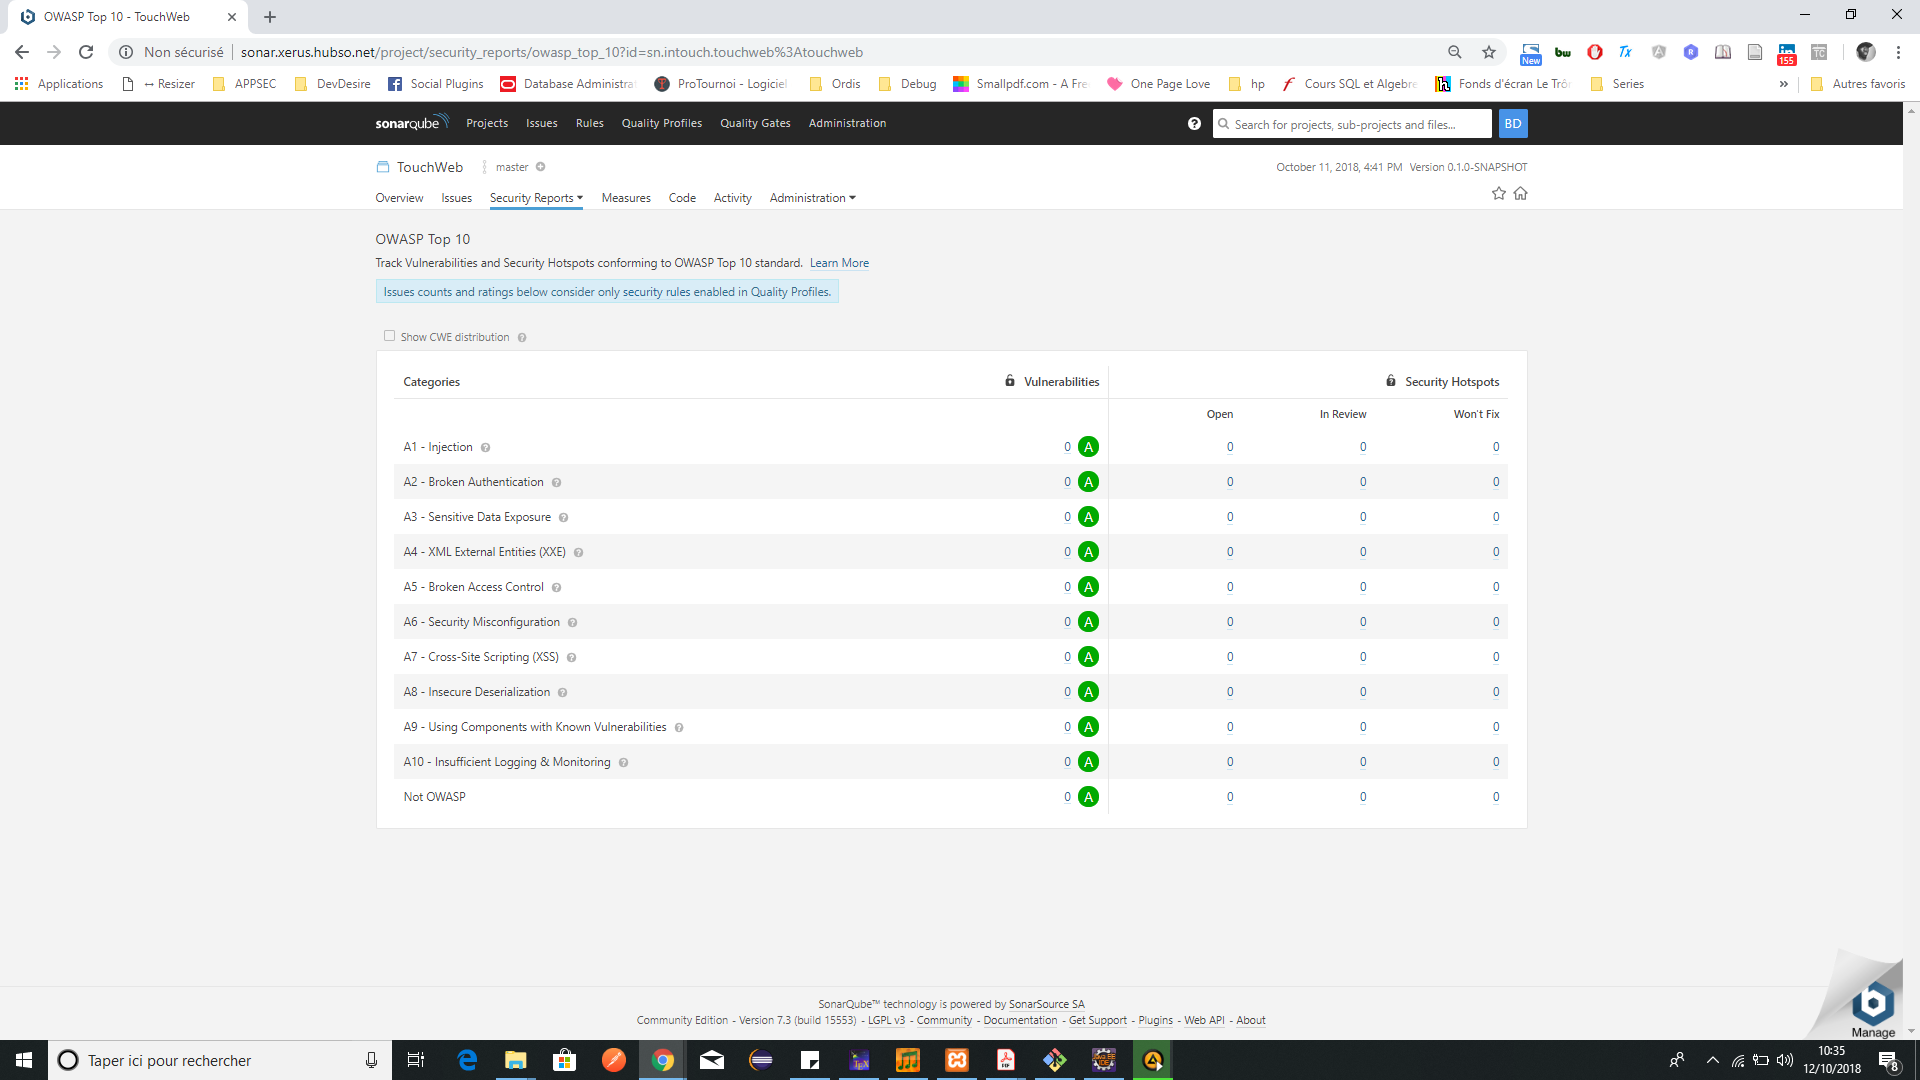
\includegraphics[width=1\textwidth]{fig/owasp_report.png}
	\end{minipage}
	\caption{Rapport Owasp Top 10}
	\label{fig:sfds}
\end{figure}